Este capítulo del trabajo tiene como objetivo detallar las diferentes partes del proceso de evaluación, desde las métricas, datasets hasta los s resultados obtenidos para los modelos y sus respectivas pruebas.

\section{Métricas} \label{metricas}
Para conocer el desempeño de nuestros modelos de forma cuantitativa es necesario evaluarlos utilizando una serie de métricas. Específicamente en tareas de clasificación como la planteada para este trabajo se consideran las más utilizadas: Accuracy,  precisión, , recall, F1-score en sus versiones macro. \cite{forman2003extensive}.

Para definir estas métricas, es necesario introducir primero los siguientes conceptos: Se entiende como Falso Positivo (en inglés, False Positive FP) como aquella instancia ha sido erróneamente clasificada como positiva por el modelo, pero que en realidad es negativa, Positivo Cierto (en inglés, True Positive, TP) como aquella instancia que es positiva y que ha sido correctamente identificada como positiva por el modelo, Falso Negativo (en inglés, False Negative, FN) como aquella instancia que aun siendo positiva, ha sido incorrectamente clasificada como negativa por el modelo y por último se entiende Cierto Negativo (en inglés, True Negative, TN) como aquella instancia negativa y que ha sido correctamente clasificada como negativa por el modelo.

\subsection{accuracy}
El accuracy mide el porcentaje de acierto de un modelo respecto al número total de instancias \cite{forman2003extensive}.

\begin{equation}
Accuracy = \frac{TP+TN}{Total}
 \label{Accuracy-Formula}
\end{equation}

\subsection{Precisión}
Se define como la proporción de verdaderos positivos con respecto a todas las predicciones positivas, incluidos los falsos positivos y los aciertos. Una baja precisión significa que nuestro modelo de aprendizaje automático produce un gran número de falsos positivos. \cite{forman2003extensive}. 

\begin{equation}
Precision = \frac{TP}{TP+FP}
 \label{Precisión-Formula}
\end{equation}


\subsection{Recall}
Recall, también conocido como tasa de verdaderos positivos (TPR), es el ratio entre el número de aciertos del modelo a la hora de aciertos a la hora de clasificar la clase positiva, y el número total de instancias de la clase positiva (es decir, entre la suma de los falsos negativos y los true positivos). \cite{forman2003extensive}.

Si nuestro modelo produce un bajo recall, significará que el número de falsos negativos (instancias positivas que no son correctamente identificadas) es muy alto. 

\begin{equation}
Recall = \frac{TP}{TP+FN}
 \label{Recall-Formula}
\end{equation}

\subsection{F1-score}
F1-score combina precisión y recall en una sola métrica para tratar de evaluar ambas métricas de manera conjunta, especialmente útil para casos en las que las dos métricas se encuentren muy separadas entre sí. Dado que la puntuación F1 es un promedio de Precisión y Recall, significa que la puntuación F1 (al menos el usado para este proyecto) otorga igual peso a Precisión y Recall \cite{forman2003extensive}. 

\begin{equation}
F1 = 2 * \frac{Precision * Recall}{Precision + Recall}
\label{F1-Score-Formula}
\end{equation}


\subsection{Macro}
Las estadísticas macro \cite{forman2003extensive} evalúan modelos entrenados para problemas de multiclasificación. Se utiliza el promedio macro en caso de desequilibrio de clase (el tamaño de instancias para cada clase es significativamente distinto). Es la media aritmética de las clases individuales relacionadas con la precisión, el recall y la puntuación F1, es decir, es la suma de todos los valores obtenidos por las diferentes clases dividido entre el número total de clases. Se utilizan puntuaciones de promedio macro cuando necesitamos tratar todas las clases por igual para evaluar el rendimiento general del clasificador frente a las etiquetas de clase más comunes.

La media macro del recall es el promedio de todos los puntajes de recall para diferentes clases. El cálculo del promedio macro sería de la siguiente forma:

\begin{equation}
RecallMacroAvg = \frac{Recall_1+Recall_2+...+Recall_n}{num clases}
\label{Recall-Macro-Avg-Formula}
\end{equation}

La media de la precisión macro es el promedio de todos los valores de precisión para las diferentes clases. El cálculo del promedio macro sería de la siguiente forma:

\begin{equation}
PreccMacroAvg = \frac{Prec_1+Prec_2+...+Prec_n}{num clases}
\label{Precision-Macro-Avg-Formula}
\end{equation}

La media de la macro F1 es el promedio de todos los valores de F1 para las diferentes clases. El cálculo del promedio macro sería de la siguiente forma:

\begin{equation}
PreccMacroAvg = \frac{F1_1+F1_2+...+F1_n}{num clases}
\label{F1-Macro-Avg-Formula}
\end{equation}

\section{Dataset} \label{dataset-study}

Durante el trabajo se dispone de una serie de datasets, todos derivados del dataset obtenido de EXIST 2023 \cite{EXIST2023} como ya se mencionó en la introducción. El objetivo fundamental durante ese subapartado será explicar las diferentes variaciones del dataset original, así como estudiar la distribución de datos dentro del mismo.

Exist proporciona un total de 6.920 + 2.076 instancias que se pueden usar para el entrenamiento de los modelos. Adicionalmente proporcionan 1.038 instancias sin clasificar usadas para entregar en la competición con las predicciones generadas, sin embargo, ese dataset no se ha usado al no participar en la competición.

Cabe destacar que de cara a la generación de modelos se planteará una división del dataset final (8896 instancias) en 3 subdatasets (train, validation y test) para seguir un proceso de aprendizaje estándar usando el sistema de validación típico. Además de esto, la subdivisión será de un 80\% de los datos para training, y un 10\% para test y validation, respectivamente. Además, estos subconjuntos se han creado de forma aleatoria, pero garantizando que la distribución de las clases no cambia de un subconjunto a otro. 

En primer lugar, cada tweet fue anotado por 6 anotadores o 'expertos'. De esta forma, cada tweet posee seis distintos veredictos, uno por cada anotador, y también para cada una de las tres subtareas (aunque este trabajo se centre únicamente en las 2 primeras tareas de clasificación binaria y multiclasificación). Es por ello por lo que, por cada tweet y por cada subtarea, hay 6 anotaciones que no son necesariamente iguales.


El formato de cada entrada del dataset es el siguiente:

\begin{enumerate}
        \item id\_EXIST: Id de la entrada.
        \item lang: Idioma del tweet.
        \item tweet: El tweet a procesar.
        \item number\_annotators: Cantidad de anotadores para el tweet (como norma son 6).
        \item annotators: Nombres identificativos para cada uno de los anotadores.
        \item gender\_annotators: Género identificativo para cada uno de los anotadores (como norma 3 mujeres y 3 hombres).
        \item age\_annotators: Franja de edad de cada anotador donde por norma suele haber 2 de cada una de las 3 franjas (18-22, 23-45, 46+).
        \item labels\_task1: Clasificación binaria sobre si es o no sexista realizada por cada anotador.
        \item labels\_task2: Multi Clasificación realizada por cada anotador en base a las clases:
            \begin{itemize}
                \item Reported.
                \item Judgmental.
                \item Direct.
                \item Unknown.
                \item “-” En caso de haber elegido como no sexista en “label\_task1”.
            \end{itemize}
        \item labels\_task3: Asignación de etiquetas por cada anotador, las etiquetas posibles son las siguientes: 
            \begin{itemize}
                \item Objectification.
                \item Sexual-violence.
                \item Stereotyping-Dominance.
                \item Ideological-Inequality.
                \item Mysoginy-Non-Sexual-Violence.
                \item “-” En caso de haber elegido como no sexista en “label\_task1”.
            \end{itemize}
        \item split: Identifica a qué split dentro del dataset pertenece.

\end{enumerate}

Para este trabajo como ya se ha mencionado la tarea número 3, asociada a la 'label\_task3' no se realizará por lo que esa fila de la entrada para todas las entradas del dataset no se tendrá en cuenta y se eliminará del estudio y transformación de los datos.

Además, las categorías annotator, gender y age se eliminan al no aportar información de cara al entrenamiento.


%\subsection{Dataset adaptado}

Para poder trabajar adecuadamente con los datos recibidos es necesario adaptar el dataset que facilite su posterior tratamiento. Se proponen dos variantes con dos objetivos claramente diferenciados: El primer dataset, cuyo objetivo es servir para el análisis de datos, se compondrá de 6 filas por cada entrada del original (una fila por anotador). De esta manera tendremos un dataset con toda la información de distribución de manera clara y precisa. A continuación, se muestra un ejemplo de conversión:

\begin{table}[H]
\begin{tabular}{|
>{\columncolor[HTML]{9B9B9B}}c |
>{\columncolor[HTML]{C0C0C0}}c |
>{\columncolor[HTML]{C0C0C0}}c |
>{\columncolor[HTML]{C0C0C0}}c |
>{\columncolor[HTML]{C0C0C0}}c |
>{\columncolor[HTML]{C0C0C0}}c |
>{\columncolor[HTML]{C0C0C0}}c |}
\hline
{\color[HTML]{000000} \textbf{Annotator}}
& \cellcolor[HTML]{9B9B9B}{\color[HTML]{000000} \textbf{1}} 
& \cellcolor[HTML]{9B9B9B}{\color[HTML]{000000} \textbf{2}}
& \cellcolor[HTML]{9B9B9B}{\color[HTML]{000000} \textbf{3}}
& \cellcolor[HTML]{9B9B9B}\textbf{4} 
& \cellcolor[HTML]{9B9B9B}\textbf{5}
& \cellcolor[HTML]{9B9B9B}\textbf{6} 
\\ \hline
{\color[HTML]{000000} \textbf{Tweet}}    
& {\color[HTML]{000000} tweet}                      
& {\color[HTML]{000000} tweet}                          
& {\color[HTML]{000000} tweet}                           
& tweet                             
& \cellcolor[HTML]{C0C0C0}tweet
& tweet                              
\\ \hline
\textbf{Task 1}                          
& YES                                      
& YES                                                   
& NO                                          
& YES                              
& NO       
& YES                            
\\ \hline
\textbf{Task 2}                          
& DIRECT                                     
& DIRECT                                                   
& \cellcolor[HTML]{C0C0C0}-                        
& DIRECT                        
& -                                 
& \cellcolor[HTML]{C0C0C0}JUDGMENTAL \\ \hline
\end{tabular}
\caption{ejemplo reducción de instancia compuesta por 6 anotadores}
\end{table}

Como se puede observar los 6 anotadores para el mismo tweet clasifican tanto la tarea 1 como la 2 de maneras diferentes entre sí, algunos coincidiendo y otros no. Para facilita el estudio de los datos esa tabla, que representa una instancia teórica del dataset generaría 6 instancias para las cuales se usaría como valor de la celda tweet el mismo valor y para las tareas 1 y 2 sus respectivos valores. 

En segundo lugar, se propone un dataset adaptado donde se reduzca la entrada observada en la tabla anterior a una sola entrada, de tal manera que para los 6 anotadores en lugar de generar 6 instancias se genere una sola. A continuación, se explica y ejemplifica el proceso:

Para las tareas 1 y 2 se cogerá el valor más repetido y en caso de empate se cogerá el que sea más común en el dataset dentro de los valores empatados. Por ejemplo, supongamos que el valor más común para la tarea 1 es 'YES' y para la tarea 2 es 'DIRECT', en caso de tener por ejemplo 2 anotadores que marquen el valor 'DIRECT' y otros dos que marcasen ' JUDGMENTAL', como han empatado a la hora de generar la nueva instancia se seleccionaría 'DIRECT' como su valor. Así como por ejemplo si se tuvieran 4 anotadores con el valor 'YES' para la tarea 1 y 2 con el valor 'NO', se elegiría el valor 'YES' para la instancia reducida.

Se muestra aquí el ejemplo ya planteado en formato tabla:

\begin{table}[H]
\begin{tabular}{|
>{\columncolor[HTML]{9B9B9B}}c |
>{\columncolor[HTML]{C0C0C0}}c |
>{\columncolor[HTML]{C0C0C0}}c |
>{\columncolor[HTML]{C0C0C0}}c |
>{\columncolor[HTML]{C0C0C0}}c |
>{\columncolor[HTML]{C0C0C0}}c |
>{\columncolor[HTML]{C0C0C0}}c |}
\hline
{\color[HTML]{000000} \textbf{Annotator}} & \cellcolor[HTML]{9B9B9B}{\color[HTML]{000000} \textbf{1}} & \cellcolor[HTML]{9B9B9B}{\color[HTML]{000000} \textbf{2}} & \cellcolor[HTML]{9B9B9B}{\color[HTML]{000000} \textbf{3}} & \cellcolor[HTML]{9B9B9B}\textbf{4} & \cellcolor[HTML]{9B9B9B}\textbf{5} & \cellcolor[HTML]{9B9B9B}\textbf{6} \\ \hline
{\color[HTML]{000000} \textbf{Tweet}}    
& {\color[HTML]{000000} tweet}                             
& {\color[HTML]{000000} tweet}                        
& {\color[HTML]{000000} tweet}                             
& tweet                             
& \cellcolor[HTML]{C0C0C0}tweet   
& tweet                             
\\ \hline
\textbf{Task 1}                        
& YES                                                     
& YES                                                     
& NO                                                      
& YES                              
& NO                  
& YES                                
\\ \hline
\textbf{Task 2}                          
& DIRECT                                                   
& DIRECT                                                   
& \cellcolor[HTML]{C0C0C0}-                                 
& JUDGMENTAL                         
& -                   
& \cellcolor[HTML]{C0C0C0}JUDGMENTAL 
\\ \hline
\end{tabular}
\caption{ejemplo reducción de instancia compuesta por 6 anotadores}
\label{not-reduced-data}
\end{table}

La instancia convertida quedaría así:

\begin{table}[H]
\begin{tabular}{|c|c|c|}
\hline
\rowcolor[HTML]{9B9B9B} 
\cellcolor[HTML]{9B9B9B}{\color[HTML]{000000} \textbf{Tweet}} 
& {\color[HTML]{000000} \textbf{Task 1}}
& {\color[HTML]{000000} \textbf{Task 2}} 
\\ \hline
\rowcolor[HTML]{C0C0C0} 
{\color[HTML]{000000} Tweet}                                
& {\color[HTML]{000000} 'YES'}          
& {\color[HTML]{000000} 'DIRECT'}        
\\ \hline
\end{tabular}
\caption{ejemplo reducción de instancia ya reducida}
\label{reduced-data}
\end{table}


%%%%%%%%%%%%%%%%%%%%%EMPIEZA AQUI EL ANÁLISIS DE BALANCES%%%%%%%%%%%%%%%%%%%%%%%
%\subsection{Análisis de datos}
A continuación se va a analizar el dataset desde el punto de vista de la distribución de los datos. En primer lugar, se desea estudiar para la primera tarea si existe alguna clase de desequilibrio en las clases sexista y no sexista dependiendo de la edad o el género.

Se plantea por tanto la siguiente hipótesis: Desde una perspectiva social es probable que exista cierto sesgo en referencia a la identificación del sexismo desde un punto de vista del género o de la edad, para demostrar o corregir esta hipótesis se muestran a continuación los siguientes gráficos:

\begin{figure}[H]
    \centering
    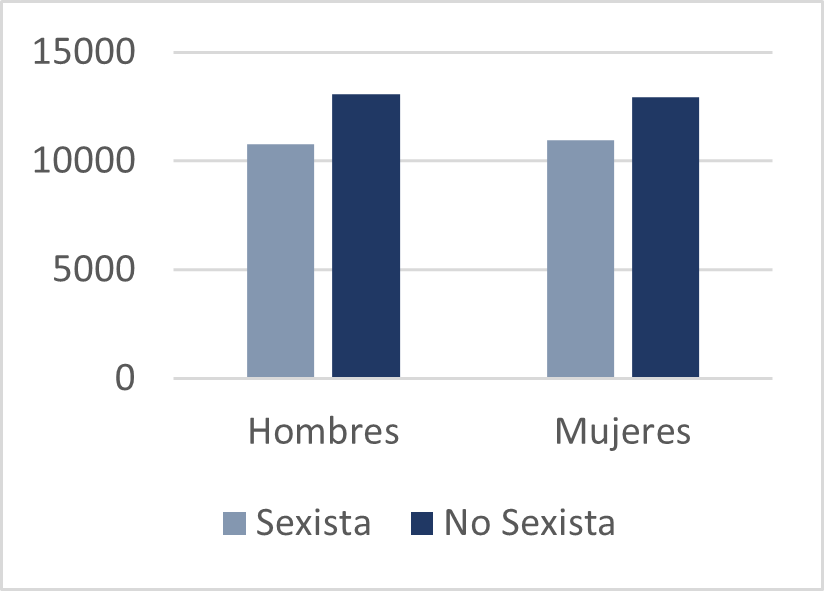
\includegraphics[width=8cm]{imagenes/Evaluacion/dataset_study/gender_task1.png}
    \caption{\centering Distribución de clases para la tarea 1 respecto del género}
    \label{gender-distribution}
\end{figure}

Se puede observar claramente que no existe un sesgo evidente desde una perspectiva del género del anotador con un total de 10.790 y 10.961 de instancias clasificadas como sexistas por hombres y mujeres respectivamente. 

A continuación se muestra la gráfica del balance de clases respecto de la edad para observar si tampoco cumple la hipótesis planteada:

\begin{figure}[H]
    \centering
    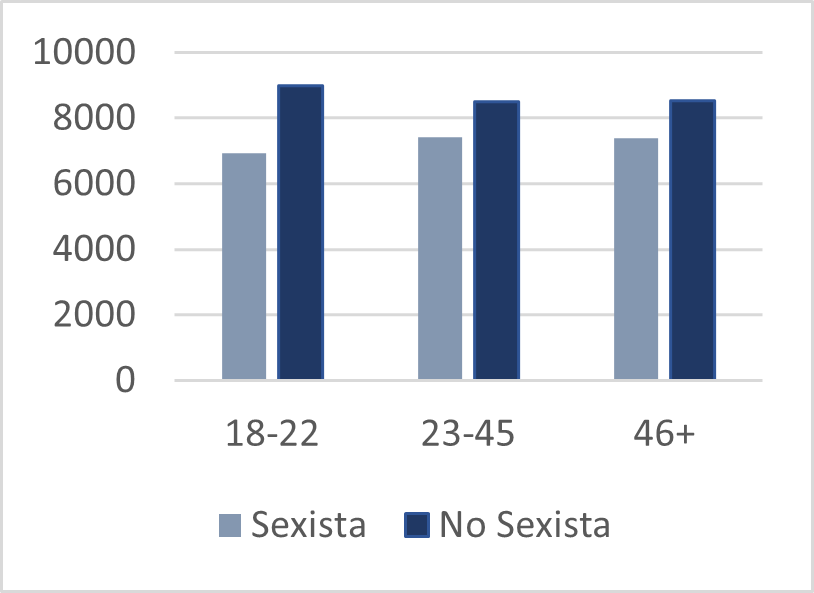
\includegraphics[width=8cm]{imagenes/Evaluacion/dataset_study/age_task1.png}
    \caption{\centering Distribución de clases para la tarea 1 respecto de la edad}
    \label{age-distribution}
\end{figure}

Si bien en este caso se observa una muy ligera tendencia por parte del grupo de edades comprendido entre 18 y 22 años a clasificar más instancias como no, no es lo suficientemente grande como para afirmar que exista un sesgo en base a la edad. Concretamente un total de 8.983 instancias fueron clasificadas como no sexistas respecto de las 8.494 y 8.520 instancias clasificadas como no sexistas por parte de los grupos de edad de 23-45 y 46+ respectivamente.

Por tanto, como se muestra claramente en \autoref{age-distribution} y en \autoref{gender-distribution} el dataset no se encuentra desbalanceado al menos desde una perspectiva de la edad o el género, desmintiendo mi hipótesis inicial.

El siguiente análisis es desde un punto de vista general de la tarea 1 y la tarea 2, como ya se ha mostrado en las tablas \autoref{reduced-data} y \autoref{not-reduced-data} la conversión de las instancias del dataset implica que para cada entrada se simplifica la opinión de 6 anotadores en una media de los mismos para ambas tareas.

Desde un punto de vista analítico esto puede favorecer el desequilibrio de las diferentes clases para cada tarea. Para realizar este análisis vamos a considerar dos datasets, uno en el que se cuenta el valor de cada anotador de forma individual (dataset base) y otro en el que se aplica la reducción ya mencionada y se compacta en una sola instancia la opinión de los 6 anotadores (dataset reducido).

Primero se analiza la distribución de clases para la tarea 1 antes y después de la reducción:

\begin{figure}[H]
    \centering
   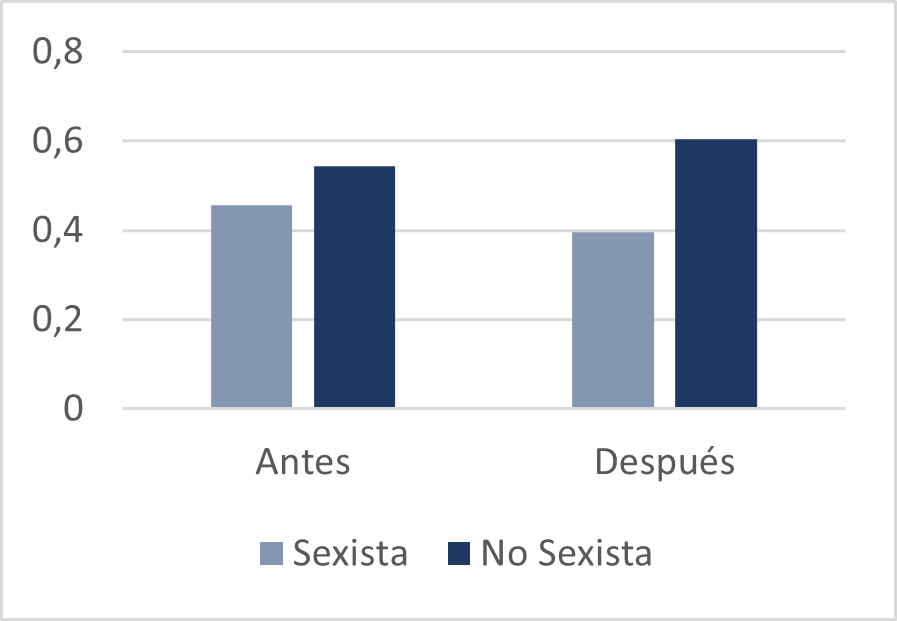
\includegraphics[width=10cm]{imagenes/Evaluacion/dataset_study/task1.png}
    \caption{\centering Distribución de clases antes y después de la reducción del dataset}
    \label{data-distribution-reducing}
\end{figure}

Una vez se realiza la reducción se pasan de tener 6 anotadores a 1 por tweet por lo que los números totales decrecen, es por eso que en lugar de mostrar en el gráfico los valores absolutos para ambas clases se muestran los valores relativos del total en cada dataset, siendo de 47.748 anotaciones respecto de las 7958 obtenidas al reducir (47.748 / 6 = 7958).

Por un lado, antes de la reducción se puede observar que ya existe un ligero desbalance en el dataset con total de 21.751 anotadores que han marcado como sexistas sus tweets respecto de los 25.997 que han marcado como no sexista sus respectivos tweets,  representando los sexistas un 45.55\% del total. Por otro lado, ese desequilibrio se incrementa al realizar la reducción (tiene sentido teniendo en cuenta el algoritmo usado para ello ejemplificado en \autoref{not-reduced-data} y \autoref{reduced-data}, obteniendo un total de 3.152 instancias clasificadas como sexistas frente a las 4.806 instancias clasificadas como no sexistas representando las sexistas un 39.6\% del total.

Es decir, de cara a la evaluación se deberá tener en cuenta el desbalance para la tarea 1 a la hora de analizar las métricas obtenidas para los modelos entrenados.

%Una vez estudiado el balance en la clase 1 se realiza el estudio para la clase 2.

Si bien para la primera tarea se plantea la hipótesis del sesgo de género o edad en base al desequilibrio de los datos, para la tarea 2 no se va a plantear ese mismo análisis. Por otro lado, si se va a estudiar el equilibrio de las diferentes clases que componen la segunda tarea, eliminando todas las instancias que pertenecen a la clase Unknown ya que como se especifica en la descripción de la tarea en \cite{EXIST2023} solo sirven para marcar cuando no se ha podido identificar el subtipo y al tratarse de una clase con solo 82 anotaciones de un total de 21.751 se consideraría ruido.

Además, se debe aclarar que los datos para la tarea 2 solo cuentan con aquellas anotaciones e instancias que hayan sido clasificadas como sexistas en la primera tarea, ya que las que no lo fueron no aportarían información al clasificar la segunda tarea como valor nulo.

De nuevo se va a estudiar el posible desequilibrio de los datos usando un gráfico con los datos antes y después de la reducción como ya se ha explicado anteriormente:

\begin{figure}[H]
    \centering
    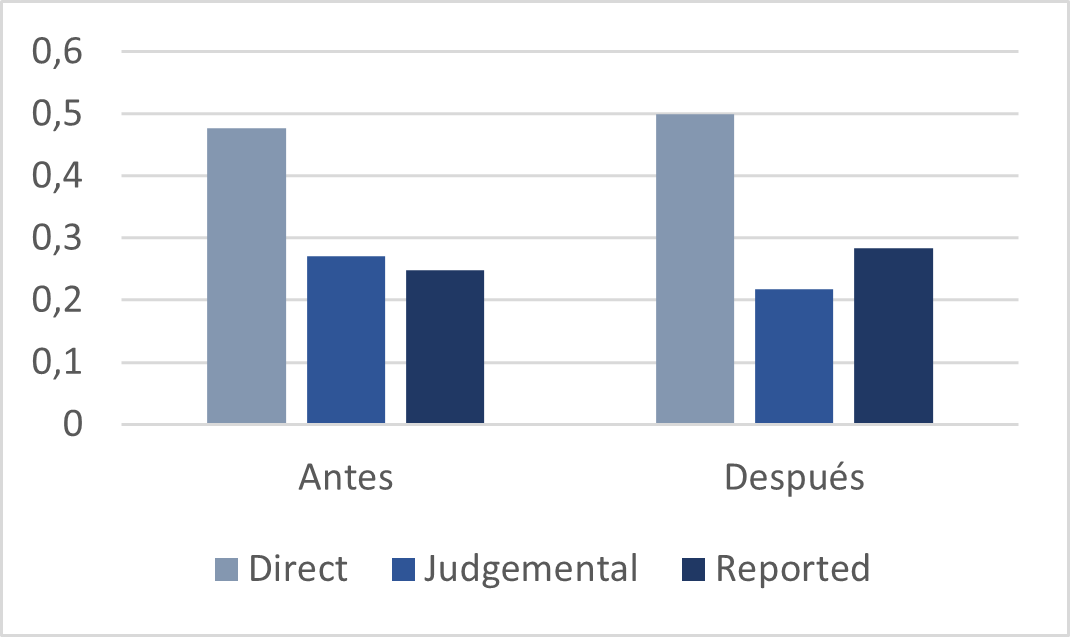
\includegraphics[width=10cm]{imagenes/Evaluacion/dataset_study/task2.png}
    \caption{\centering Balance de clases para la tarea 2 antes y después de la reducción del dataset base}
    \label{balance-task2}
\end{figure}

Por un lado, para los datos antes de la reducción se observa que la clase mayoritaria es claramente la clase Direct con un total de 10.382 anotaciones respecto de las 5.878 y 5.409 anotaciones de las clases Judgemental y Reported respectivamente. Estos resultados representan las siguientes proporciones del total: Un 47,73\% para Direct, un 27,02\% para Judgemental y un 24,86\% para Reported.

Por otro lado, una vez realizada la reducción se observa que la clase mayoritaria sigue siendo la clase Direct con un total de 1575 instancias, seguido de la clase Reported con 892 instancias y Judgemental con 684 instancias. Estos resultados representan las siguientes proporciones del total: Un 49,96\% para Direct, un 21,70\% para Judgemental y un 28,29\% para Reported.

Es decir, antes y después de la reducción la clase Direct compone alrededor del 50\% de los datos, mientras que las otras dos clases componen alrededor del 25\% cada una, sin embargo después de la reducción se ha observado que las clases Judgemental y Reported cambian sus porcentajes pasando Reported de un 24.86\% a un 28.29\% y Judgemental de un 27,02\% a un 21,70\%.

De nuevo habrá que tener en cuenta a la hora de evaluar los resultados obtenidos para los diferentes modelos el desequilibrio entre las diferentes clases para analizar un correcto estudio de los resultados.

%\subsection{Tamaño de tweets}

Además de estudiar la distribución de las clases, se desea estudiar el tamaño de los tweets, considerando como tamaño el número de tokens en el tweet. 

La tabla \ref{tab:lengthtexts} muestra un histograma con la distribución de los tamaños de los tweets. Siendo los valores máximos y mínimos 3 y 78 respectivamente, además de la media de 28,19 tokens. Se puede observar claramente que aproximadamente el 75\% de los tweets se encuentran alrededor de los 40 tokens. 

\begin{figure}[H]
    \centering
    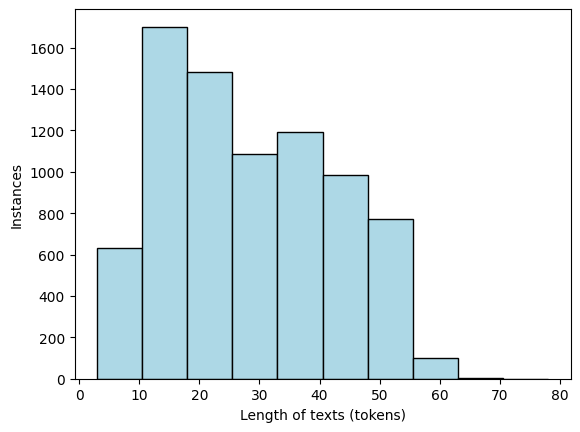
\includegraphics[width=10cm]{imagenes/Evaluacion/dataset_study/lenght_all_tokens.png}
    \caption{\centering Histograma de la longitud de los textos (número de tokens)}
    \label{tab:lengthtexts}
\end{figure}

También se pueden observar unos valores alejados de la media y del centro de gravedad del histograma, pero no se consideran destacables al representar una clara minoría del dataset.

A continuación, se estudia el tamaño de los tweets en base a su clasificación, tanto para la tarea 1 como para la tarea 2. Nuestro objetivo es estudiar si el tamaño de los textos está relacionado con si el tweet es o no sexista, y en el caso de la tarea 2, si está relacionado con el tipo de contenido sexista. Para la tarea 2, la distribución se estudia únicamente sobre el conjunto de tweets clasificados como sexistas como ya se ha comentado anteriormente. 


\begin{figure}[H]
    \centering
    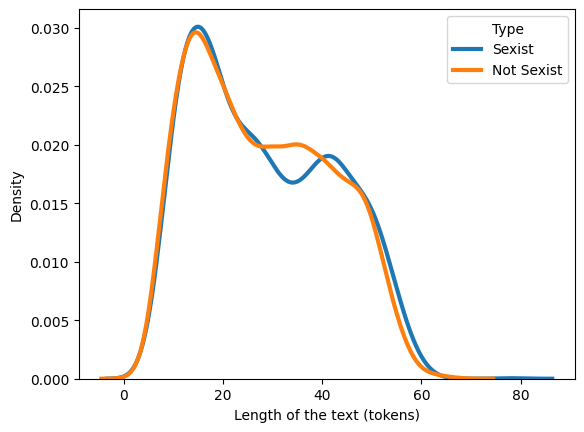
\includegraphics[width=10cm]{imagenes/Evaluacion/dataset_study/sexist_not_sexist_tokens.png}
    \caption{\centering Distribución del tamaño de los tweets (tokens) diferenciando entre tweets sexistas y no sexistas}
    \label{fig:sexist_not_sexist}
\end{figure}

Se puede observar que no existen diferencias destacables en el tamaño de los tweets en relación a si son sexistas o no (Figura \ref{fig:sexist_not_sexist}).

\begin{figure}[H]
    \centering
    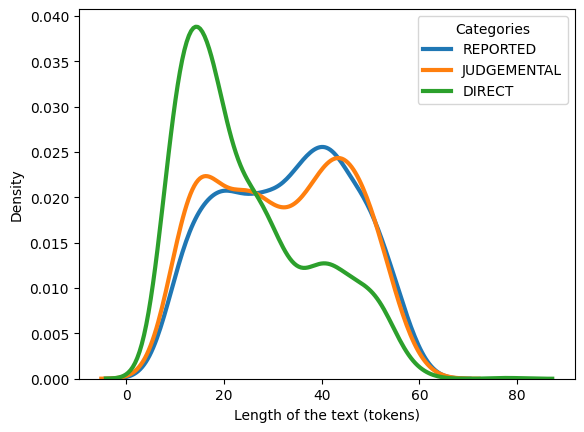
\includegraphics[width=10cm]{imagenes/Evaluacion/dataset_study/task2_lenght_tokens.png}
    \caption{\centering Distribución del tamaño de los tweets (tokens) con contenido sexista en relación a las clases de la tarea 2}
    \label{fig:task2_lenght}

\end{figure}

En la figura \ref{fig:task2_lenght} podemos observar que los tweets clasificados como Direct tienen una tendencia bastante clara a ser más cortos en comparación con los tweets Judgemental y los Reported. Dicho eso, se plantea la siguiente hipótesis: probablemente se debe al carácter inherente de los tweets clasificados como Direct, cuyo objetivo probablemente es simplemente ofender o buscar el agravio sexista, a diferencia de los otros dos que buscan hablar sobre el tema de manera más extendida, aunque esto es solo una hipótesis, y se debería realizar un análisis más detallado sobre los tweets de cada tipo, para poder comprender esta diferencia. 

Para ejemplificar esto se muestran los siguientes tweets, tanto en español como en inglés, donde se puede ver que el tamaño de los tweets Direct es significativamente menor que el de las clases Reported y Judgemental:

\begin{itemize}
    \item Tweet 201073 (Direct): White liberal feminism is a cancer {URL}
    \item Tweet 201075 (Reported): @User1 @User2 No he's just perpetuating the lie that feminism is funded by  Catholic evangelilical sponsors from the US sic. This lie is a direct assault on womens right and ability to self organise. The attack on Catholism is more to do with the Church's history of  rape of its flock.
    \item Tweet 201089 (Judgemental): I laugh at how Celia and her clan pretend to be these great Feminists when in reality they’ve excluded and bullied other women in the house (i.e. Anahi and Alicia)…In celia’s words to Alicia 'I hope that bitch vomits blood' who the fuck even says that unprovoked \#LCDLF
    \item Tweet 100008 (Direct): @User Esta gringa sigue llorando por el gamergate, que 'coincidencia' que tenga pronombres en su perfil
    \item Tweet (Reported): @User1 @User2 @User3 Pues mira no, son hombres, cada uno con su familia, amistades y haciendo vida normal. Igual que los de LaManada, y los que asesinan a diario a sus parejas. Por eso deberíamos preguntarnos qué coño está pasando con los hombres para q actúen así, y qué clase de sociedad queremos.
    \item Tweet (Judgemental): @User1 @User2 @User3 Entonces como así es el mercado lo mejor no es hacer algo para cambiarlo y seguir alimentando el machismo en los consumidores en lugar apoyar a gente como las víctimas del gamergate.Acerca de lo otro, el 'tenían' implica un imperativo entonces no entiendo lo del buscaban.
\end{itemize}



Una vez realizado el preprocesado de los datos siguiendo el esquema planteado en \autoref{preprocesado}, se podrían estudiar de nuevo las diferentes distribuciones dentro del dataset. Sin embargo, se ha observado que las proporciones no varían por lo que solo se va a mostrar el gráfico con el número de tokens al considerar los otros redundantes.

\begin{figure}[H]
    \centering
    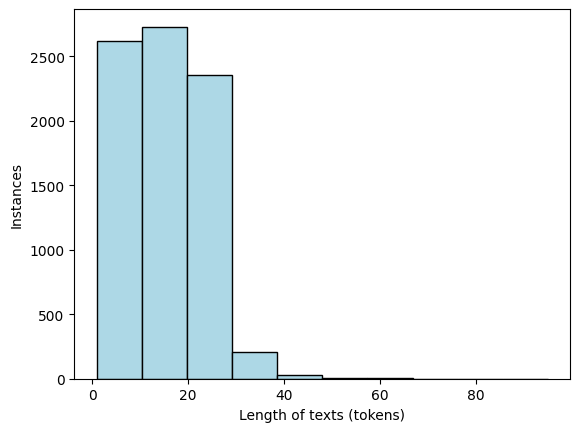
\includegraphics[width=10cm]{imagenes/Evaluacion/dataset_study/preprocessed_text_lenght_tokens.png}
    \caption{\centering Distribución de tamaños en función del número de caracteres preprocesada}
\end{figure}

Lo primero que se puede observar es la bajada en los valores, por un lado sus valores mínimo y máximo se sitúa en 1 y 95 así como su media se sitúa en 15,53 tokens. En segundo lugar, los tweets se han equilibrado alrededor de los valores 9 y 20 a diferencia de \autoref{tab:lengthtexts} cuyos tamaños se encontraban más distribuidos.

\section{Resultados para la tarea de clasificación binaria}
Durante esta sección se van a explicar los diferentes resultados obtenidos para los diferentes modelos planteados en \autoref{cap:modelos}. Realizando de manera adicional un breve análisis sobre aquellos mejores modelos, sus fortalezas, debilidades y posibles razones por las que han obtenido esos resultados.

Tal y como se explicó en el capítulo \ref{cap:modelos}, cada uno de los modelos fue entrenado con distintas versiones del conjunto de entrenamiento: todos los tweets tanto en español como en inglés, ii) únicamente tweets en inglés, iii) todos los tweets preprocesados, y iv) tweets en inglés preprocesados. El objetivo es comparar resultados entre entrenar un modelo utilizando todos los textos disponibles en el dataset (tanto en inglés como en español), y además estudiar el efecto del preprocesado sobre los resultados finales. 

Antes de comenzar es importante destacar el objetivo de este estudio, se desean comparar los modelos para textos en inglés aplicados a una tarea multilingüe respecto de modelos multilingües, para ello se proporcionan resultados tanto solo para los textos en inglés (como referencia) así como para la totalidad de los textos.

\subsection{Bert Base Cased}
El primero de los modelos elegidos es el modelo base de Bert con la variante Cased, la cual recordando, esencialmente trabaja con el dataset original sin quitar todas las mayúsculas. Este modelo suele ser utilizado para tareas como reconocimiento de entidades, donde las mayúsculas y minúsculas si son importantes para discernir si un token o frase son una entidad. Además, es necesario recordar que este modelo fue preentrenado únicamente utilizando textos en inglés. A continuación, se muestran los resultados obtenidos para las cuatro variantes ya mencionadas:

\begin{table}[H]
\begin{tabular}{|c|l|l|l|l|}
\hline
\rowcolor[HTML]{9B9B9B} 
{\color[HTML]{000000} \textbf{Versión}} 
& \multicolumn{1}{c|}{\cellcolor[HTML]{9B9B9B}{\color[HTML]{000000} \textbf{Accuracy}}} 
& \multicolumn{1}{c|}{\cellcolor[HTML]{9B9B9B}{\color[HTML]{000000} \textbf{F1}}} 
& \multicolumn{1}{c|}{\cellcolor[HTML]{9B9B9B}{\color[HTML]{000000} \textbf{Precisión}}} 
& \multicolumn{1}{c|}{\cellcolor[HTML]{9B9B9B}{\color[HTML]{000000} \textbf{Recall}}} 
\\ \hline
\rowcolor[HTML]{E7E6E6} 
\cellcolor[HTML]{9B9B9B}{\color[HTML]{000000} \textbf{Todos los tweets sin preprocesar}}  
& {\color[HTML]{000000} 0.785}  
& {\color[HTML]{000000} 0.775}  
& {\color[HTML]{000000} 0.771}  
& {\color[HTML]{000000} 0.780}                                                     
\\ \hline
\rowcolor[HTML]{E7E6E6} 
\cellcolor[HTML]{9B9B9B}{\color[HTML]{000000} \textbf{Tweets en ingles sin preprocesar}}  
& {\color[HTML]{000000} 0.810} 
& {\color[HTML]{000000} 0.797}                                                 
& {\color[HTML]{000000} 0.794} 
& {\color[HTML]{000000} 0.801}                                                     
\\ \hline
\rowcolor[HTML]{E7E6E6} 
\cellcolor[HTML]{9B9B9B}{\color[HTML]{000000} \textbf{Todos los tweets preprocesados}} 
& {\color[HTML]{000000} 0.765} 
& {\color[HTML]{000000} 0.752}                                                 
& {\color[HTML]{000000} 0.750}                                                    
& {\color[HTML]{000000} 0.756}                                                     
\\ \hline
\rowcolor[HTML]{E7E6E6} 
\cellcolor[HTML]{9B9B9B}{\color[HTML]{000000} \textbf{Tweets en inglés preprocesados}}                                                  
& {\color[HTML]{000000} 0.760}                                                    
& {\color[HTML]{000000} 0.748}                                                 
& {\color[HTML]{000000} 0.744}                                                    
& {\color[HTML]{000000} 0.759}                                                    
\\ \hline
\end{tabular}
\caption{Resultados para Bert-base-cased sobre el conjunto de test.}
\label{bert-base-cased-results}
\end{table}

Se observa una clara tendencia por parte de los modelos no preprocesados a obtener mejores resultados respecto de sus contrapartes con preprocesamiento con unos valores de accuracy 0.785 y 0.810 para los sin preprocesar bilingües e ingleses respectivamente frente a los valores de 0.765 y 0.760 de sus versiones con preprocesado.

En general queda claro que el mejor modelo generado con esta variante es el modelo que solo contiene tweets en inglés lo cual es coherente al tratarse Bert-base de un modelo preentrenado únicamente con textos en inglés. Por tanto, ajustar el modelo para la tarea con también tweets en español no ayuda a mejorar los resultados. 


Además, cabe destacar que, pese a no estar entrenado con textos en castellano, los resultados son bastante buenos respecto de los resultados en inglés, con diferencias muy pequeñas entre los resultados utilizando la colección completa o únicamente utilizando los tweets en inglés. La misma conclusión se obtienen cuando los tweets son preprocesados.

\subsection{Bert Base Uncased}
El segundo de los modelos elegidos es la variación del anterior para el formato uncased donde se ignoraban las mayúsculas y se procesaba todo el texto en minúsculas sin hacer distinción entre palabras iguales con o sin mayúsculas. Posee también un entrenamiento solo en inglés, pero con un uso más genérico y no especializado en entidades como su contraparte.

\begin{table}[H]
\begin{tabular}{|c|l|l|l|l|}
\hline
\rowcolor[HTML]{9B9B9B} 
{\color[HTML]{000000} \textbf{Versión}}  
& \multicolumn{1}{c|}{\cellcolor[HTML]{9B9B9B}{\color[HTML]{000000} \textbf{Accuracy}}} 
& \multicolumn{1}{c|}{\cellcolor[HTML]{9B9B9B}{\color[HTML]{000000} \textbf{F1}}} 
& \multicolumn{1}{c|}{\cellcolor[HTML]{9B9B9B}{\color[HTML]{000000} \textbf{Precision}}} 
& \multicolumn{1}{c|}{\cellcolor[HTML]{9B9B9B}{\color[HTML]{000000} \textbf{Recall}}} 
\\ \hline
\rowcolor[HTML]{E7E6E6} 
\cellcolor[HTML]{9B9B9B}{\color[HTML]{000000} \textbf{Todos los tweets sin preprocesar}}                                                                 
& {\color[HTML]{000000} 0.765}                                                    
& {\color[HTML]{000000} 0.750}                                                 
& {\color[HTML]{000000} 0.749}                                                    
& {\color[HTML]{000000} 0.750}                                                     
\\ \hline
\rowcolor[HTML]{E7E6E6} 
\cellcolor[HTML]{9B9B9B}{\color[HTML]{000000} \textbf{Tweets en ingles sin preprocesar}}                                                  
& {\color[HTML]{000000} 0.741}                                                       
& {\color[HTML]{000000} 0.723}                                                 
& {\color[HTML]{000000} 0.724}                                                        
& {\color[HTML]{000000} 0.721}                                                     
\\ \hline
\rowcolor[HTML]{E7E6E6} 
\cellcolor[HTML]{9B9B9B}{\color[HTML]{000000} \textbf{Todos los tweets preprocesados}}                                                  
& {\color[HTML]{000000} 0.808}                                                   
& {\color[HTML]{000000} 0.800}                                                
& {\color[HTML]{000000} 0.797}                                                    
& {\color[HTML]{000000} 0.819}                                                    
\\ \hline
\rowcolor[HTML]{E7E6E6} 
\cellcolor[HTML]{9B9B9B}{\color[HTML]{000000} \textbf{Tweets en inglés preprocesados}}                                                 
& {\color[HTML]{000000} 0.808}                                                   
& {\color[HTML]{000000} 0.797}                                                 
& {\color[HTML]{000000} 0.792}                                                    
& {\color[HTML]{000000} 0.807}                                                    
\\ \hline
\end{tabular}
\caption{Resultados para Bert-base-uncased sobre el conjunto de test.}
\label{bert-base-uncased-results}
\end{table}


El modelo uncased obtiene mejores resultados que el modelo cased, lo cual es consistente con nuestras conclusiones anteriores. Por tanto, transformar los textos de entrada a minúsculas, permite generalizar mejor y obtener mejores resultados en una tarea de clasificación como esta. En contraposición con los modelos generados para la variante Cased, para Bert uncased se observa que aquellos modelos con preprocesado obtienen resultados significativamente mejores, superándolos con una clara mejora en sus valores de F1 del 5\% para el modelo base y un 7.4\% para el modelo en inglés.

Si bien dentro de los preprocesados, parece que el base obtiene mejores resultados respecto del inglés, cabe destacar un doble factor a tener en cuenta. Por un lado, el dataset para tweets en inglés es significativamente más pequeño por lo que eso puede afectar ligeramente al aprendizaje al tener menor capacidad de generalización y por otro lado las diferencias en resultados no alcanzan ni el 1\% por lo que no se pueden considerar realmente significativas.

\subsection{Bert Base Multilingual}
Los siguientes modelos buscan mejorar los resultados respecto de los modelos de bert-base que contienen tanto los tweets en español como en inglés. Para ello se plantea Bert Base Multilingual usando tanto la variante cased \cite{bert-base-multilingual-cased} como la variante uncased \cite{bert-base-multilingual-uncased} para tener una mayor fuente de datos para analizar. 

En este caso solo se estudian los datasets que contienen todos los tweets ya que no se busca observar las mejoras respecto del inglés, sino las mejoras respecto del total que incluye los tweets en español realizando así el análisis de capacidades multilingües ya mencionado.

\begin{table}[H]
\begin{tabular}{|c|l|l|l|l|}
\hline
\rowcolor[HTML]{9B9B9B} 
{\color[HTML]{000000} \textbf{Versión}} 
& \multicolumn{1}{c|}{\cellcolor[HTML]{9B9B9B}{\color[HTML]{000000} \textbf{Accuracy}}} 
& \multicolumn{1}{c|}{\cellcolor[HTML]{9B9B9B}{\color[HTML]{000000} \textbf{F1}}} 
& \multicolumn{1}{c|}{\cellcolor[HTML]{9B9B9B}{\color[HTML]{000000} \textbf{Precision}}}
& \multicolumn{1}{c|}{\cellcolor[HTML]{9B9B9B}{\color[HTML]{000000} \textbf{Recall}}} 
\\ \hline
\rowcolor[HTML]{E7E6E6} 
\cellcolor[HTML]{9B9B9B}{\color[HTML]{000000} \textbf{Cased}}                           
& {\color[HTML]{000000} 0.767}                                                  
& {\color[HTML]{000000} 0.753}                                      
& {\color[HTML]{000000} 0.752}                                               
& {\color[HTML]{000000} 0.754}                                                     
\\ \hline
\rowcolor[HTML]{E7E6E6} 
\cellcolor[HTML]{9B9B9B}{\color[HTML]{000000} \textbf{Preprocesado Cased}}   
                                               
& {\color[HTML]{000000} 0.772}                                                       
& {\color[HTML]{000000} 0.763}                                                 
& {\color[HTML]{000000} 0.759}                                                        
& {\color[HTML]{000000} 0.770}                                                     
\\ \hline
\rowcolor[HTML]{E7E6E6} 
\cellcolor[HTML]{9B9B9B}{\color[HTML]{000000} \textbf{Uncased}}              
                                                  
& {\color[HTML]{000000} 0.788}                                                       
& {\color[HTML]{000000} 0.774}                                                 
& {\color[HTML]{000000} 0.775}                                                        
& {\color[HTML]{000000} 0.773}                                                     
\\ \hline
\rowcolor[HTML]{E7E6E6} 
\cellcolor[HTML]{9B9B9B}{\color[HTML]{000000} \textbf{Preprocesado Uncased}} 
                                               
& {\color[HTML]{000000} 0.746}                                                      
& {\color[HTML]{000000} 0.730}                                                 
& {\color[HTML]{000000} 0.729}                                                        
& {\color[HTML]{000000} 0.731}                                                     
\\ \hline
\end{tabular}
\caption{Resultados para Bert-base-multilingual sobre el conjunto de test.}
\end{table}

Se observa una caída en los resultados para el dataset preprocesado para el modelo uncased siendo completamente al revés para el modelo cased, algo que ya se había podido observar en \autoref{bert-base-cased-results} y \autoref{bert-base-uncased-results}. Adicionalmente se observa claramente que el mejor modelo es el que no recibe preprocesamiento y se genera usando el modelo Uncased con unos valores F1 de 0.774 y accuracy de 0.788, además de unos valores en las demás métricas muy similares.

Por otro lado, para los dos modelos generados con Cased se observan apenas ninguna diferencia entre ambos (alrededor del 1\%). 

Queda por tanto claro que el mejor modelo generado con la versión multilingüe es creado usando el modelo uncased sin preprocesamiento, pudiendo observar quizás una ligera tendencia por parte de los modelos a obtener mejores resultados cuando no se preprocesa el dataset. Esto se estudiará más adelante.


\subsection{Roberta Base}
El siguiente modelo es Roberta, como ya se ha comentado Roberta es un modelo basado en BERT, que fue entrenado usando grandes colecciones de textos que incluían textos de redes sociales. Por ello se considera que se pueden obtener resultados interesantes en la tarea planteada, aunque sus textos de entrenamiento sean exclusivamente en inglés.

\begin{table}[H]
\begin{tabular}{|c|l|l|l|l|}
\hline
\rowcolor[HTML]{9B9B9B} 
{\color[HTML]{000000} \textbf{Versión}}                                     
& \multicolumn{1}{c|}{\cellcolor[HTML]{9B9B9B}{\color[HTML]{000000} \textbf{Accuracy}}}
& \multicolumn{1}{c|}{\cellcolor[HTML]{9B9B9B}{\color[HTML]{000000} \textbf{F1}}}
& \multicolumn{1}{c|}{\cellcolor[HTML]{9B9B9B}{\color[HTML]{000000} \textbf{Precision}}} 
& \multicolumn{1}{c|}{\cellcolor[HTML]{9B9B9B}{\color[HTML]{000000} \textbf{Recall}}} 
\\ \hline
\rowcolor[HTML]{E7E6E6} 
\cellcolor[HTML]{9B9B9B}{\color[HTML]{000000} \textbf{Todos los tweets sin preprocesar}}                                                             
& {\color[HTML]{000000} 0.783}                                                     
& {\color[HTML]{000000} 0.772}                                               
& {\color[HTML]{000000} 0.770}                                           
& {\color[HTML]{000000} 0.776}                                                  
\\ \hline
\rowcolor[HTML]{E7E6E6} 
\cellcolor[HTML]{9B9B9B}{\color[HTML]{000000} \textbf{Tweets en inglés sin preprocesar}}                                                
& {\color[HTML]{000000} 0.781}                                                     
& {\color[HTML]{000000} 0.777}                                              
& {\color[HTML]{000000} 0.785}                                                   
& {\color[HTML]{000000} 0.809}                                                 
\\ \hline
\rowcolor[HTML]{E7E6E6} 
\cellcolor[HTML]{9B9B9B}{\color[HTML]{000000} \textbf{Todos los tweets preprocesados}}                                                        
& {\color[HTML]{000000} 0.767}                                                     
& {\color[HTML]{000000} 0.740}                                                
& {\color[HTML]{000000} 0.760}                                                  
& {\color[HTML]{000000} 0.731}                                                    
\\ \hline
\rowcolor[HTML]{E7E6E6} 
\cellcolor[HTML]{9B9B9B}{\color[HTML]{000000} \textbf{Tweets en inglés preprocesados}}                                            
& {\color[HTML]{000000} 0.797}                                                    
& {\color[HTML]{000000} 0.785}                                                
& {\color[HTML]{000000} 0.780}                                                      
& {\color[HTML]{000000} 0.793}                                                  
\\ \hline
\end{tabular}
\caption{Resultados para Roberta-base sobre el conjunto de test.}
\label{roberta-base-results}
\end{table}

En estos resultados se puede observar claramente que de nuevo los modelos sin preprocesamiento se comportan mejor que los que si tienen preprocesamiento como ya ha pasado anteriormente. Por un lado, el modelo para los tweets en ingles sin preprocesar obtiene unos valores de F1 de 0.777 y Accuracy de 0.781, y el modelo multilingüe obtiene unos cercanos 0.772 y 0.783 de F1 y Accuracy respectivamente. Sin embargo, sus valores de recall se encuentran algo separados con un 0.775 para el base y un 0.809 para el base en inglés, es decir, el modelo en inglés tiene una mayor capacidad para identificar positivos y no pasarlos por alto como falsos negativos respecto del otro.

Se puede determinar que el mejor modelo para RoBERTa es el modelo base en inglés con unos valores de accuracy y precisión de 0.781 y 0.785 respectivamente lo cual se mantiene coherente al tratarse de un modelo de nuevo creado para tareas en inglés.

\subsection{Twitter RoBERTa base emotion}
El siguiente modelo, Twitter RoBERTa base emotion \cite{twitter-roberta-base-emotion} es una variante de RoBERTa que como ya se ha comentado ha sido ajustada específicamente para el análisis de sentimientos con datos de Twitter. Por ello se considera que puede ofrecer resultados interesantes para nuestra tarea y se ha usado como modelo adicional dentro de Roberta.

\begin{table}[H]
\begin{tabular}{|c|l|l|l|l|}
\hline
\rowcolor[HTML]{9B9B9B} 
{\color[HTML]{000000} \textbf{Versión}}                                    
& \multicolumn{1}{c|}{\cellcolor[HTML]{9B9B9B}{\color[HTML]{000000} \textbf{Accuracy}}}
& \multicolumn{1}{c|}{\cellcolor[HTML]{9B9B9B}{\color[HTML]{000000} \textbf{F1}}}
& \multicolumn{1}{c|}{\cellcolor[HTML]{9B9B9B}{\color[HTML]{000000} \textbf{Precision}}}
& \multicolumn{1}{c|}{\cellcolor[HTML]{9B9B9B}{\color[HTML]{000000} \textbf{Recall}}} 
\\ \hline
\rowcolor[HTML]{E7E6E6} 
\cellcolor[HTML]{9B9B9B}{\color[HTML]{000000} \textbf{Todos los tweets sin preprocesar}}                                                           
& {\color[HTML]{000000} 0.771}                                                     
& {\color[HTML]{000000} 0.754}                                             
& {\color[HTML]{000000} 0.756}                                                    
& {\color[HTML]{000000} 0.752}                                                
\\ \hline
\rowcolor[HTML]{E7E6E6} 
\cellcolor[HTML]{9B9B9B}{\color[HTML]{000000} \textbf{Tweets en inglés sin preprocesar}}                                             
& {\color[HTML]{000000} 0.829}                                                    
& {\color[HTML]{000000} 0.816}                                            
& {\color[HTML]{000000} 0.813}                                                   
& {\color[HTML]{000000} 0.819}                                                   
\\ \hline
\rowcolor[HTML]{E7E6E6} 
\cellcolor[HTML]{9B9B9B}{\color[HTML]{000000} \textbf{Todos los tweets preprocesados}}                                                       
& {\color[HTML]{000000} 0.766}                                                   
& {\color[HTML]{000000} 0.742}                                            
& {\color[HTML]{000000} 0.755}                                                      
& {\color[HTML]{000000} 0.735}                                               
\\ \hline
\rowcolor[HTML]{E7E6E6} 
\cellcolor[HTML]{9B9B9B}{\color[HTML]{000000} \textbf{Tweets en inglés sin preprocesados}}                                           
& {\color[HTML]{000000} 0.784}                                                      
& {\color[HTML]{000000} 0.762}                                                
& {\color[HTML]{000000} 0.766}                                                     
& {\color[HTML]{000000} 0.759}                                                     
\\ \hline
\end{tabular}
\caption{Resultados para Twitter-RoBERTa-base-emotion sobre el conjunto de test.}
\end{table}

Lo primero que se puede observar de manera clara y directa es que los resultados el modelo base en inglés son los mejores hasta el momento con unos valores de 0.829 y 0.816 de Accuracy y F1 respectivamente. Teniendo en cuenta que este modelo se ha entrenado con una base de datos de tweets en inglés tiene bastante sentido observar estos resultados.

Por otro lado, las métricas para el modelo base no son para nada malas, de hecho, se sitúan en la parte superior en calidad respecto del resto de modelos ya estudiados. Es interesante ver como modelos preentrenados con tweets son capaces claramente de adaptarse y trabajar con mayor facilidad con el dataset.

Además, de nuevo se vuelve a observar como aquellos modelos que no poseen preentrenamiento sobre los datos obtienen mejores resultados respecto de aquellos que sí.

\subsection{XLM-Roberta-base}
XLM-Roberta \cite{xlm-roberta} es el equivalente multilingüe de RoBERTa, ofreciendo en la teoría una capacidad de generar modelos con varios lenguajes a la vez, superior a la que ofrecía RoBERTa como ya se había comentado. El objetivo es observar si existen mejoras respecto de su contraparte para alguna de las 4 versiones generadas y en caso de existir considerarlas para la solución final.

Una característica reseñable de XLM es su entrenamiento, como ya se mencionó en apartados anteriores, basado en aproximadamente textos de 100 lenguajes diferentes, siendo el inglés y el castellano los idiomas con mayor número de textos.

\begin{table}[H]
\begin{tabular}{|c|l|l|l|l|}
\hline
\rowcolor[HTML]{9B9B9B} 
{\color[HTML]{000000} \textbf{Versión}}                                    
& \multicolumn{1}{c|}{\cellcolor[HTML]{9B9B9B}{\color[HTML]{000000} \textbf{Accuracy}}} 
& \multicolumn{1}{c|}{\cellcolor[HTML]{9B9B9B}{\color[HTML]{000000} \textbf{F1}}}
& \multicolumn{1}{c|}{\cellcolor[HTML]{9B9B9B}{\color[HTML]{000000} \textbf{Precision}}} 
& \multicolumn{1}{c|}{\cellcolor[HTML]{9B9B9B}{\color[HTML]{000000} \textbf{Recall}}} 
\\ \hline
\rowcolor[HTML]{E7E6E6} 
\cellcolor[HTML]{9B9B9B}{\color[HTML]{000000} \textbf{Todos los tweets sin preprocesar}}                                              
& {\color[HTML]{000000} 0.782}                                                    
& {\color[HTML]{000000} 0.775}                                             
& {\color[HTML]{000000} 0.772}                                   
& {\color[HTML]{000000} 0.786}                                                
\\ \hline
\rowcolor[HTML]{E7E6E6} 
\cellcolor[HTML]{9B9B9B}{\color[HTML]{000000} \textbf{Tweets en inglés sin preprocesar}}                                      
& {\color[HTML]{000000} 0.765}                                                      
& {\color[HTML]{000000} 0.751}                             
& {\color[HTML]{000000} 0.747}                            
& {\color[HTML]{000000} 0.759}                                         
\\ \hline
\rowcolor[HTML]{E7E6E6} 
\cellcolor[HTML]{9B9B9B}{\color[HTML]{000000} \textbf{Todos los tweets preprocesados}}                                    
& {\color[HTML]{000000} 0.736}                                                     
& {\color[HTML]{000000} 0.724}            
& {\color[HTML]{000000} 0.721}                                                   
& {\color[HTML]{000000} 0.729}                                                 
\\ \hline
\rowcolor[HTML]{E7E6E6} 
\cellcolor[HTML]{9B9B9B}{\color[HTML]{000000} \textbf{Tweets en inglés preprocesados}} 

& {\color[HTML]{000000} 0.757}                                                                                            
& {\color[HTML]{000000} 0.744}                                   
& {\color[HTML]{000000} 0.740}                                         
& {\color[HTML]{000000} 0.753}                                   
\\ \hline
\end{tabular}
\caption{Resultados para XLM-RoBERTa-base sobre el conjunto de test.}
\end{table}

En general los resultados obtenidos son peores en todos los aspectos respecto de los resultados de RoBERTa mostrados en la \autoref{roberta-base-results}. Concretamente el único que obtiene resultados similares es el modelo creado con todos los tweets sin preprocesar con unos valores de F1 y Accuracy de 0.754 y 0.771 respectivamente. 

Eso sí, de igual manera que para los demás modelos se observa que aquellos modelos generados con los datos preprocesados obtienen peores valores respecto de aquellos que no han recibido preprocesamiento.

\subsection{Mejores modelos}

Durante este apartado se van a comparar directamente los mejores modelos encontrados durante las diferentes pruebas realizadas para la tarea de clasificación binaria. Los modelos se han obtenidos de los ya analizados y por ende este apartado solo tiene como objetivo determinar de manera clara y analítica cuales son los 2 mejores modelos finales para su análisis. 

Cabe destacar que se realizará una subdivisión final en la que, de esos dos modelos, uno se elegirá entre los modelos bilingües y otro se elegirá de los modelos únicamente ingleses. De esta manera se tendrá una perspectiva clara sobre las capacidades de los modelos presentados basados en bert para trabajar con idiomas diferentes del inglés.

A continuación, se muestran los mejores modelos solo con tweets en inglés:

\begin{table}[H]
\begin{tabular}{|l|l|l|l|l|}
\hline
\rowcolor[HTML]{9B9B9B} 
\multicolumn{1}{|c|}{\cellcolor[HTML]{9B9B9B}{\color[HTML]{000000} \textbf{Versión}}}      
& \multicolumn{1}{c|}{\cellcolor[HTML]{9B9B9B}{\color[HTML]{000000} \textbf{Accuracy}}}
& \multicolumn{1}{c|}{\cellcolor[HTML]{9B9B9B}{\color[HTML]{000000} \textbf{F1}}} 
& \multicolumn{1}{c|}{\cellcolor[HTML]{9B9B9B}{\color[HTML]{000000} \textbf{Precision}}}
& \multicolumn{1}{c|}{\cellcolor[HTML]{9B9B9B}{\color[HTML]{000000} \textbf{Recall}}} 
\\ \hline
\rowcolor[HTML]{E7E6E6} 
\cellcolor[HTML]{9B9B9B}{\color[HTML]{000000} \textbf{Bert-base-cased inglés}}                                                           
& {\color[HTML]{000000} 0.8106}                                                
& {\color[HTML]{000000} 0.7973}                                             
& {\color[HTML]{000000} 0.7940}                                 
& {\color[HTML]{000000} 0.8018}                                                 
\\ \hline
\rowcolor[HTML]{E7E6E6} 
\cellcolor[HTML]{9B9B9B}{\color[HTML]{000000} \textbf{Bert-base-uncased Inglés}}                                                       
& {\color[HTML]{000000} 0.808}                                              
& {\color[HTML]{000000} 0.800}                                                
& {\color[HTML]{000000} 0.797}                                                    
& {\color[HTML]{000000} 0.819}                                                   
\\ \hline
\rowcolor[HTML]{E7E6E6} 
\cellcolor[HTML]{9B9B9B}{\color[HTML]{000000} \textbf{Roberta-base inglés}}                                                            
& {\color[HTML]{000000} 0.781}                                               
& {\color[HTML]{000000} 0.777}                                           
& {\color[HTML]{000000} 0.785}                                            
& {\color[HTML]{000000} 0.809}                                                   
\\ \hline
\rowcolor[HTML]{E7E6E6} 
\cellcolor[HTML]{9B9B9B}{\color[HTML]{000000} \textbf{Twitter-roberta-base-emotion inglés}}                                            
& {\color[HTML]{000000} 0.821}                                                       
& {\color[HTML]{000000} 0.809}                                              
& {\color[HTML]{000000} 0.805}                                                      
& {\color[HTML]{000000} 0.816}                                                   
\\ \hline
\end{tabular}
\caption{Mejores modelos primera tarea solo tweets en inglés.}
\end{table}

En general, podemos observar que los modelos se encuentran alrededor del 80\% de media para las diferentes métricas estudiadas. Esto se cumple salvo para un modelo, el mejor de ellos de hecho, el modelo basado en Roberta y twitter 'Twitter-roberta-base-emotion'. Este modelo de todos los planteados era de manera teórica el más consistente con el dataset de este trabajo y por ende era esperable que fuera el que mejor resultados obtuviera al menos de cara a los tweets en inglés. Concretamente ha obtenido unos valores de 0.821 y 0.809 para Accuracy y F1 respectivamente.

A continuación, se muestran sus diferentes métricas desglosadas en un formato donde poder analizar de manera más precisa sus resultados, mostrando los valores obtenidos tanto de forma general como para cada label de manera específica, así como la media ponderada de las mismas:

\begin{table}[H]
\begin{tabular}{|
>{\columncolor[HTML]{9B9B9B}}l |
>{\columncolor[HTML]{E7E6E6}}l |
>{\columncolor[HTML]{E7E6E6}}l |
>{\columncolor[HTML]{E7E6E6}}l |}
\hline
\multicolumn{1}{|c|}{\cellcolor[HTML]{9B9B9B}{\color[HTML]{000000} \textbf{Versión}}}
& \multicolumn{1}{c|}{\cellcolor[HTML]{9B9B9B}{\color[HTML]{000000} \textbf{F1}}} 
& \multicolumn{1}{c|}{\cellcolor[HTML]{9B9B9B}{\color[HTML]{000000} \textbf{Precision}}} 
& \multicolumn{1}{c|}{\cellcolor[HTML]{9B9B9B}{\color[HTML]{000000} \textbf{Recall}}}
\\ \hline
{\color[HTML]{000000} \textbf{No Sexista}}                                 
& {\color[HTML]{000000} 0.85}                                                
& {\color[HTML]{000000} 0.88}                                                            
& {\color[HTML]{000000} 0.81}                                                         
\\ \hline
{\color[HTML]{000000} \textbf{Sexista}}                                           
& {\color[HTML]{000000} 0.75}                                                 
& {\color[HTML]{000000} 0.71}                                                        
& {\color[HTML]{000000} 0.81}                                                         
\\ \hline
{\color[HTML]{000000} \textbf{Weighted Average}}                                   
& {\color[HTML]{000000} 0.81}                                                    
& {\color[HTML]{000000} 0.82}                                                     
& {\color[HTML]{000000} 0.81}                                                    
\\ \hline
\end{tabular}
\caption{Métricas desglosadas Twitter-roberta-base-emotion.}
\end{table}

Antes de comenzar es importante mencionar el uso de medias ponderadas para las métricas desglosadas con el objetivo de tener una visión en conjunto de los resultados desde un punto de vista relativo y no absoluto.

Los resultados del conjunto de pruebas indican que el modelo tiene un rendimiento bastante bueno para la tarea de clasificación binaria, con una puntuación de F1 de 0.75 para sexista y 0.85 para No Sexista. Además, la precisión es razonablemente alta para ambos casos, con una precisión de 0.71 para sexista y 0.88 para No Sexista. El recall también es bastante bueno para ambos casos, con un recall de 0.78 para sexista y 0.76 para No Sexista.

Se puede observar una ligera tendencia hacia clasificar el 'no' correctamente, esto se puede deber al tratarse de la clase mayoritaria en el dataset. De no tenerse en cuenta esto podría llevar a mayores errores en el futuro como sobre entrenamiento, pero de cara a estas pruebas no se considera una tara lo suficientemente grande como para considerarla un problema.

Por último, para comprobar la teoría planteada se va a estudiar brevemente la matriz de confusión generada usando YES para sexista y NO para No Sexista:

\begin{figure}[H]
    \centering
    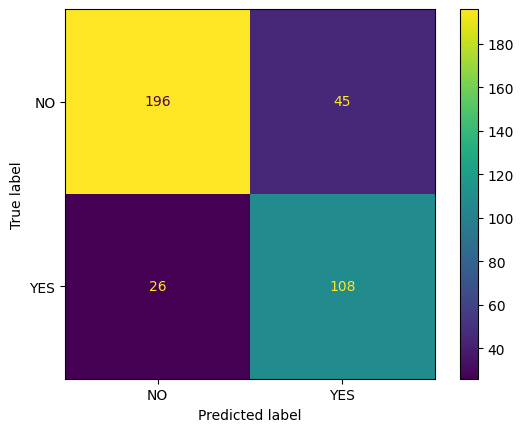
\includegraphics[width=10cm]{imagenes/Evaluacion/confusion_matrix/twitter_roberta_base_emotion-english-dirty.png}
    \caption{\centering matriz de confusión para TWITTER-ROBERTA-BASE-EMOTION}
\end{figure}


Se puede observar inmediatamente que se han clasificado correctamente 196 instancias de la etiqueta No Sexista, así como 108 de Sexista. Por el otro lado, para Sexista se observan un total de 26 instancias mal clasificadas respecto del total de 134 (un 19\%) y para No Sexista se observan 45 instancias mal clasificadas de un total de 241 (un 19\%) pudiendo determinar que si bien en las métricas se observan ciertas tendencias al No Sexista como ya se teorizaba, en la matriz de confusión no se observan evidencias de ello. En conclusión, tras analizar la matriz de confusión, así como las diferentes métricas se obtiene para este modelo un accuracy del 81.06\%.

Por el otro lado tenemos los mejores modelos para la tarea en su formato bilingüe:

\begin{table}[H]
\begin{tabular}{|l|l|l|l|l|}
\hline
\rowcolor[HTML]{9B9B9B} 
\multicolumn{1}{|c|}{\cellcolor[HTML]{9B9B9B}{\color[HTML]{000000} \textbf{Versión}}} 
& \multicolumn{1}{c|}{\cellcolor[HTML]{9B9B9B}{\color[HTML]{000000} \textbf{Accuracy}}} 
& \multicolumn{1}{c|}{\cellcolor[HTML]{9B9B9B}{\color[HTML]{000000} \textbf{F1}}} 
& \multicolumn{1}{c|}{\cellcolor[HTML]{9B9B9B}{\color[HTML]{000000} \textbf{Precision}}} 
& \multicolumn{1}{c|}{\cellcolor[HTML]{9B9B9B}{\color[HTML]{000000} \textbf{Recall}}} 
\\ \hline
\rowcolor[HTML]{E7E6E6} 
\cellcolor[HTML]{9B9B9B}{\color[HTML]{000000} \textbf{Bert-base-cased}}                                                              
& {\color[HTML]{000000} 0.785}                                                     
& {\color[HTML]{000000} 0.775}                                                 
& {\color[HTML]{000000} 0.771}                                                       
& {\color[HTML]{000000} 0.780}                                                   
\\ \hline
\rowcolor[HTML]{E7E6E6} 
\cellcolor[HTML]{9B9B9B}{\color[HTML]{000000} \textbf{Bert-base-multilingual-uncased}}                                                  
& {\color[HTML]{000000} 0.788}                                                    
& {\color[HTML]{000000} 0.774}                                                
& {\color[HTML]{000000} 0.775}                                                          
& {\color[HTML]{000000} 0.773}                                                   
\\ \hline
\rowcolor[HTML]{E7E6E6} 
\cellcolor[HTML]{9B9B9B}{\color[HTML]{000000} \textbf{Twitter-roberta-base-emotion}}                                               
& {\color[HTML]{000000} 0.771}                                        
& {\color[HTML]{000000} 0.754}                                               
& {\color[HTML]{000000} 0.756}                         
& {\color[HTML]{000000} 0.752}                                         
\\ \hline
\rowcolor[HTML]{E7E6E6} 
\cellcolor[HTML]{9B9B9B}{\color[HTML]{000000} \textbf{XLM-roBERTa}}                                       
& {\color[HTML]{000000} 0.782}                                              
& {\color[HTML]{000000} 0.775}                                            
& {\color[HTML]{000000} 0.772}                                                
& {\color[HTML]{000000} 0.786}                                                 
\\ \hline
\end{tabular}
\caption{Mejores modelos primera tarea bilingüe.}
\end{table}

Para estos resultados observamos unos números muy similares entre los modelos salvo para el modelo generado con twitter-roberta-base-emotion que se obtienen peores resultados, todos los demás rondando el 78\% en todas las métricas. Es decir, se sitúan algo por debajo de los mejores en inglés como era de esperar. 

Si hubiera que elegir un mejor modelo, aunque no sea por mucho el mejor modelo es el generado por Bert multilingüe uncased, probablemente debido a su arquitectura y su capacidad de generalizar en varios idiomas es lo que le permite obtener unos mejores resultados, aunque estos no sean significativamente mejores que los demás modelos.

A continuación, se muestran sus diferentes métricas desglosadas en un formato donde poder analizar de manera más precisa sus resultados, mostrando los valores obtenidos tanto de forma general como para cada label de manera específica, así como la media ponderada de las mismas:

\begin{table}[H]
\begin{tabular}{|
>{\columncolor[HTML]{9B9B9B}}l |
>{\columncolor[HTML]{E7E6E6}}l |
>{\columncolor[HTML]{E7E6E6}}l |
>{\columncolor[HTML]{E7E6E6}}l |}
\hline
\multicolumn{1}{|c|}{\cellcolor[HTML]{9B9B9B}{\color[HTML]{000000} \textbf{Versión}}} 
& \multicolumn{1}{c|}{\cellcolor[HTML]{9B9B9B}{\color[HTML]{000000} \textbf{F1}}} 
& \multicolumn{1}{c|}{\cellcolor[HTML]{9B9B9B}{\color[HTML]{000000} \textbf{Precision}}} 
& \multicolumn{1}{c|}{\cellcolor[HTML]{9B9B9B}{\color[HTML]{000000} \textbf{Recall}}} 
\\ \hline
{\color[HTML]{000000} \textbf{No Sexista}}                                              
& {\color[HTML]{000000} 0.82}                                                    
& {\color[HTML]{000000} 0.79}                                                        
& {\color[HTML]{000000} 0.85}                                                        
\\ \hline
{\color[HTML]{000000} \textbf{Sexista}}                                             
& {\color[HTML]{000000} 0.71}                                                    
&{\color[HTML]{000000} 0.75}                                                    
& {\color[HTML]{000000} 0.68}                                               
\\ \hline
{\color[HTML]{000000} \textbf{Weighted Average}}                                  
& {\color[HTML]{000000} 0.78}                                              
& {\color[HTML]{000000} 0.78}                                                  
& {\color[HTML]{000000} 0.78}                                                         
\\ \hline
\end{tabular}
\caption{Métricas Bert-multilingual-uncased.}
\end{table}

Se puede ver claramente en la tabla como el modelo tiende a clasificar mejor los textos no sexistas respecto de los sexistas con unos valores de F1 de 0.82 y 0.71 respectivamente. También es interesante destacar como la clase Sexista tiene un recall muy bajo de 0.68 por lo que se asume que tiene una alta tendencia a clasificar falsos sexistas.

En resumen, el modelo tiene una clara tendencia a clasificar mejor los tweets no sexistas que los sexistas, esto tiene sentido recordando las proporciones del dataset y el posible mayor aprendizaje para detectar no sexistas. Esto además se puede observar aún mejor con el valor de recall de 0.85.

Por último, para comprobar las conclusiones planteadas, se va a estudiar brevemente la matriz de confusión generada del conjunto de test:

\begin{figure}[H]
    \centering
    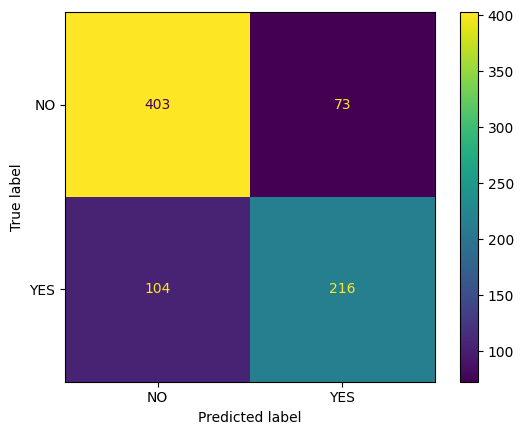
\includegraphics[width=10cm]{imagenes/Evaluacion/confusion_matrix/bert_base_multilingual-uncased-all-dirty.png}
    \caption{\centering matriz de confusión para bert-multilingual-uncased}
\end{figure}

En comparación con la matriz de confusión para la versión inglesa se observan ciertas disparidades en los resultados. En primera instancia si bien la clase No Sexista tiene un total de 73 instancias mal clasificadas de un total de 476 (un 15\%), la clase Sexista posee 104 instancias mal clasificadas de un total de 320, presentando un 33\% de error doblando al producido con su contraparte. 

Con toda esta información, se demuestra que en este entrenamiento sí que ha habido desequilibrio de clases con una clara tendencia a la clase 'No' lo cual se puede deber al aumento significativo en el número de instancias de entrenamiento lo que puede favorecer el desequilibrio hacia la clase mayoritaria. En conclusión, tras analizar la matriz de confusión, así como las diferentes métricas se obtiene para este modelo un accuracy del 77.76\%.


\section{Modelos segunda tarea}

Para la segunda tarea se plantea un estudio a menor escala en comparación usando los modelos ya marcados como buenos para este dataset en la tarea 1. Estos modelos servirán para ofrecer una perspectiva de las limitaciones y capacidades de los modelos bert para generar resultados una vez la tarea se complica como pasa con la segunda tarea.


\subsection{Análisis previo}
El principal hándicap de la segunda tarea consiste en la subclasificación dentro de las clases Judgemental y Reported. Estas dos clases poseen un parecido intrínseco en su composición y características al menos desde un punto de vista humano.

A continuación, se realiza una pequeña demostración del problema principal planteado mostrando una serie de tweets, sin decir cuál es su clasificación dentro de Judgemental y Reported. En primera instancia se usarán 4 tweets en español para ejemplificarlo: 

\begin{enumerate}
        \item Tweet 100038: Encima siempre a la misma pobre tisi she’s being harassed
        \item Tweet 100005: Entonces como así es el mercado lo mejor no es hacer algo para cambiarlo y seguir alimentando el machismo en los consumidores en lugar apoyar a gente como las víctimas del gamergate.Acerca de lo otro, el 'tenían' implica un imperativo entonces no entiendo lo del buscaban.
        \item Tweet 100042: Pues mira no, son hombres, cada uno con su familia, amistades y haciendo vida normal. Igual que los de LaManada, y los que asesinan a diario a sus parejas. Por eso deberíamos preguntarnos qué coño está pasando con los hombres para q actúen así, y qué clase de sociedad queremos.
        \item Tweet 100060: Lo de Lopetegui en rueda de prensa diciendo no sé qué de la minifalda y tal... Era por los de \#LaManada... No?.
\end{enumerate}

%Esos 4 tweets pertenecen 2 a una clase y 2 a la otra y, sin embargo, parecen pertenecer a las dos clases de manera simultánea al no ser realmente capaz de diferenciar que los convierte en Judgemental o en Reported. 

Podemos ver que entre los seis anotadores existen discrepancias a la hora de anotar cada uno de los tweets anteriores.
%Si matizamos en el problema de base y se analiza el dataset original con los 6 anotadores originales se empiezan a observar cosas interesantes. 

Por ejemplo, el tweet 100005 posee cuatro anotadores que detectan como sexismo el tweet, de esos cuatro anotadores, uno declara que es sexismo directo, mientras otros dos declaran que es sexismo de juicio (Judgemental) y uno que es una situación de reporte.

Con el resto de tweets, podemos observar que tampoco  hay una unanimidad clara respecto de esas dos subclases. Por lo que cabe preguntarse si realmente existen tantas diferencias sustanciales entre ambas clases.

A continuación, se realiza el mismo estudio, pero con 4 tweets en inglés:


\begin{enumerate}
        \item Tweet 200623: Even most women who are having trouble because they put off kids for too long weren't riding the cock carousel, they were hyperfocused on their careers. Often were married the whole time.
        \item Tweet 200709: You are a woman and you are allowing another woman cook for your husband and wash his clothes too, even as far as clean and dress the room, some women don't like their marriages sha
        \item Tweet 200714: Hardest thing about being a wife is figuring out what to cook for your husband. And he said no Asian food sad face emoji
        \item Tweet 200766: There aren't. In your study they were 31\%, in mine there were 44.9\%.I don't know that they do, what does it have to do with me?Trans men are much less visible than trans women due to discrimination. I don't see how that proves we're the bad guys.
\end{enumerate}

De nuevo se observa el patrón ya mencionado siendo realmente complicado identificar la clase de cada tweet, y dar argumentos sólidos de por qúe. No solo eso, si observamos de nuevo qué valores dan los 6 anotadores se puede observar, por ejemplo, que para el tweet 200623, 5 anotadores que detectaron sexismo, dos marcaron que era de juicio, otros 2 que era un reporte y uno solo que era directo.

En conclusión, existen claras discrepancias entre los anotadores, y por tanto, es normal que los modelos tengan dificultades a la hora de distinguir entre Judgemental y Reported. Esto se suma al desequilibrio ya comentado dentro de las 3 clases donde alrededor del 50\% de las instancias pertenecen a Direct donde Judgemental y Reported tienen alrededor de un 25\% de las instancias (ver análisis de datos).

\subsection{Modelos en inglés}

A continuación, se muestran los 4 modelos escogidos para el estudio de clasificación sobre el dataset con solo tweets en inglés. Estos 4 modelos se han escogido como ya se ha mencionado en base a los 4 mejores para la anterior tarea para los tweets en inglés. En teoría se esperan resultados significativamente peores que para la primera tarea y una clara tara a la hora de clasificar las dos subclases ya mencionadas:

\begin{table}[H]
\begin{tabular}{|l|l|l|l|l|}
\hline
\rowcolor[HTML]{9B9B9B} 
\multicolumn{1}{|c|}{\cellcolor[HTML]{9B9B9B}{\color[HTML]{000000} \textbf{Versión}}} 
& \multicolumn{1}{c|}{\cellcolor[HTML]{9B9B9B}\textbf{Accuracy}} 
& \multicolumn{1}{c|}{\cellcolor[HTML]{9B9B9B}\textbf{F1}}
& \multicolumn{1}{c|}{\cellcolor[HTML]{9B9B9B}\textbf{Precision}} 
& \multicolumn{1}{c|}{\cellcolor[HTML]{9B9B9B}\textbf{Recall}} 
\\ \hline
\rowcolor[HTML]{E7E6E6} 
\cellcolor[HTML]{9B9B9B}\textbf{bert\_base-cased}                                                            
& {\color[HTML]{000000} 0.609}                              
& {\color[HTML]{000000} 0.533}                         
& {\color[HTML]{000000} 0.536}                              
& {\color[HTML]{000000} 0.531}                            
\\ \hline
\rowcolor[HTML]{E7E6E6} 
\cellcolor[HTML]{9B9B9B}\textbf{bert\_base-uncased}                                                          
& {\color[HTML]{000000} 0.616}                               
& {\color[HTML]{000000} 0.619}                        
& {\color[HTML]{000000} 0.620}                              
& {\color[HTML]{000000} 0.619}                           
\\ \hline
\rowcolor[HTML]{E7E6E6} 
\cellcolor[HTML]{9B9B9B}\textbf{roberta-base}                                                               
& {\color[HTML]{000000} 0.601}                               
& {\color[HTML]{000000} 0.541}                         
& {\color[HTML]{000000} 0.541}                               
& {\color[HTML]{000000} 0.541}                            
\\ \hline
\rowcolor[HTML]{E7E6E6} 
\cellcolor[HTML]{9B9B9B}\textbf{twitter\_roberta\_base\_emotion}                                           
& {\color[HTML]{000000} 0.609}                             
& {\color[HTML]{000000} 0.521}                       
& {\color[HTML]{000000} 0.530}                               
& {\color[HTML]{000000} 0.513}                             
\\ \hline
\end{tabular}
\caption{Métricas de los modelos en inglés segunda tarea.}
\end{table}

Para una tarea con tanto desbalance de datos como se pudo observar en la \autoref{balance-task2}, es imperativo usar como referencia para la calidad de los modelos el valor de F1 al ofrecer una perspectiva conjunta de tanto el Recall como la Precision como ya se explicó en la \autoref{metricas}.

De primeras se puede observar claramente que el mejor modelo en todas las métricas es bert\_base\_uncased con u valor de F1 de 0.619. Sin embargo, el modelo twitter\_roberta\_base\_emotion del cual se esperarían resultados al menos mínimamente aceptables obtiene el peor valor de F1 de todos los modelos con un 0.521.

Durante el entrenamiento se observó algo inusual que se desea estudiar, el valor de loss para el modelo generado con bert\_base\_uncased estaba muy por encima del valor de los demás a diferencia del modelo twitter\_roberta\_base\_emotion cuyo valor de loss se encontraba radicalmente por debajo del resto. Si bien en modelos con el mismo dataset esto debería indicar que el mejor modelo es el segundo, en la tabla se observan resultados completamente distintos.

Es por esto que en lugar de analizar exclusivamente el modelo bert\_base\_uncased se van a estudiar tanto ese modelo como el twitter\_roberta\_base\_emotion para tratar de entender a qué se puede deber esa clara disparidad en su entrenamiento.

\subsection{Mejores modelos inglés: Bert\_base-uncased}

Estas secciones tienen como objetivo analizar las diferencias entre los dos modelos seleccionados en el apartado anterior, bert\_base-uncased y twitter\_roberta\_base\_emotion. Con ello se pretende esclarecer las diferentes incógnitas generadas con la primera aproximación al estudio de la segunda tarea como las diferencias en los valores de loss y las diferentes métricas.

En primer lugar, se analizan los resultados obtenidos para el modelo bert\_base-uncased sobre el set de test, de nuevo usando la media ponderada ya mencionada en apartados anteriores: 

\begin{table}[H]
\begin{tabular}{|l|c|c|c|c|}
\hline
\rowcolor[HTML]{9B9B9B} 
\multicolumn{1}{|c|}{\cellcolor[HTML]{9B9B9B}{\color[HTML]{000000} \textbf{Versión}}} 
& \multicolumn{1}{l|}{\cellcolor[HTML]{9B9B9B}{\color[HTML]{000000} \textbf{Direct}}} 
& \multicolumn{1}{l|}{\cellcolor[HTML]{9B9B9B}{\color[HTML]{000000} \textbf{Judgemental}}}
& \multicolumn{1}{l|}{\cellcolor[HTML]{9B9B9B}{\color[HTML]{000000} \textbf{Reported}}}
& \multicolumn{1}{l|}{\cellcolor[HTML]{9B9B9B}{\color[HTML]{000000} \textbf{Weighted Average}}} 
\\ \hline
\rowcolor[HTML]{E7E6E6} 
\cellcolor[HTML]{9B9B9B}{\color[HTML]{000000} \textbf{F1}}                           
& {\color[HTML]{000000} 0.66}                                                        
& {\color[HTML]{000000} 0.40}                                                         
& {\color[HTML]{000000} 0.32}                                                             
& {\color[HTML]{000000} 0.52}                                                          
\\ \hline
\rowcolor[HTML]{E7E6E6} 
\cellcolor[HTML]{9B9B9B}{\color[HTML]{000000} \textbf{Precision}}                    
& {\color[HTML]{000000} 0.74}                                                       
& {\color[HTML]{000000} 0.30}                                                      
& {\color[HTML]{000000} 0.47}                                                        
& {\color[HTML]{000000} 0.57}                                                     
\\ \hline
\rowcolor[HTML]{E7E6E6} 
\cellcolor[HTML]{9B9B9B}{\color[HTML]{000000} \textbf{Recall}}                      
& {\color[HTML]{000000} 0.59}                                                       
& {\color[HTML]{000000} 0.60}                                                        
& {\color[HTML]{000000} 0.24}                                                         
& {\color[HTML]{000000} 0.51}                                                        
\\ \hline
\end{tabular}
\caption{Métricas segunda tarea bert\_base-uncased inglés.}
\end{table}

De nuevo para observar los resultados globales la métrica interesante es F1, sin embargo tanto Precision como Recall nos ofrecen información muy útil del modelo. Por un lado, la clase Direct, claramente la mejor clase en cuanto a resultados ofrece un valor de precisión de 0.74, es decir con una tasa de acierto alta cuando predice que un valor pertenece a su clase, pero por el contrario su valor de recall cae a 0.59 sugiriendo que confunde muchas entradas como si fueran de otra de las clases.

Se acaba de mencionar que la clase Direct tiene una razonable tendencia a clasificar como otra clase las entradas que le pertenecen. La clase Judgemental tiene unos valores de Precision y recall de 0.47 y 0.24 respectivamente, así como la clase Reported tiene 0.30 y 0.60 respectivamente. 

Estos valores tan bajos sugieren dos cosas, por un lado que efectivamente muchos de los valores de la clase mayoritaria Direct se están clasificando como una de estas dos y por otro lado que este modelo tiene un claro desajuste a la hora de clasificar con una alta calidad comparado con las otras dos clases para Direct.

Para poder avanzar en el análisis se ofrece a continuación una perspectiva distinta con la matriz de confusión:

\begin{figure}[H]
    \centering
    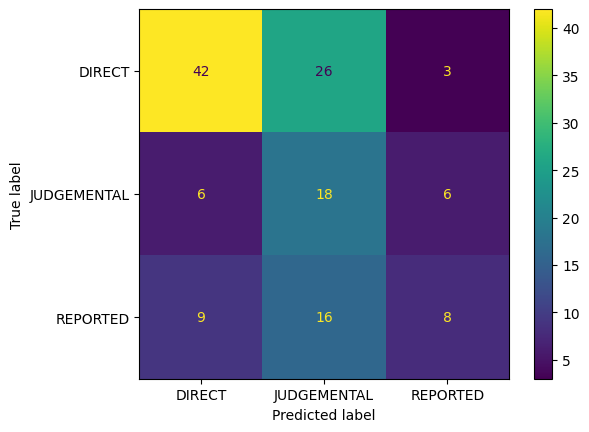
\includegraphics[width=10cm]{imagenes/Evaluacion/confusion_matrix/bert_base-uncased-english-dirty_task2.png}
    \caption{\centering matriz de confusión para bert-base-uncased}
\end{figure}

Para la primera clase se observan un total de 42 instancias bien clasificadas frente al total de 71, es decir un 59.15\%. Por el otro lado las clases Reported y Judgemental tienen 18 y 8 instancias bien clasificadas lo que supone un 60\% y 24.24\% respectivamente. 

Es decir, se puede observar una tendencia por parte del modelo a clasificar hacia la clase Reported con un total de 60 instancias clasificadas como Reported frente a las solo 15 instancias de Judgemental. Esto se puede deber a diversos factores como por ejemplo la hipótesis planteada al inicio sobre la similitud intrínseca de las entradas de tipo Judgemental y de tipo Reported. Es, por tanto, sin duda una tara característica del modelo. Adicionalmente cabe destacar que de manera global el modelo obtiene un 50.7\% de tasa de acierto.


\subsection{Mejores modelos inglés: Twitter\_roberta\_base\_emotion}

A continuación, se ofrecen los resultados para el modelo generado con twitter\_roberta\_base\_emotion, con el cual se desea observar sus valores respecto del modelo  bert\_base-uncased para tratar de determinar si existe alguna causa para esos valores tan dispares.

\begin{table}[H]
\begin{tabular}{|l|c|c|c|c|}
\hline
\rowcolor[HTML]{9B9B9B} 
\multicolumn{1}{|c|}{\cellcolor[HTML]{9B9B9B}{\color[HTML]{000000} \textbf{Versión}}} 
& \multicolumn{1}{l|}{\cellcolor[HTML]{9B9B9B}{\color[HTML]{000000} \textbf{Direct}}} 
& \multicolumn{1}{l|}{\cellcolor[HTML]{9B9B9B}{\color[HTML]{000000} \textbf{Judgemental}}}
& \multicolumn{1}{l|}{\cellcolor[HTML]{9B9B9B}{\color[HTML]{000000} \textbf{Reported}}}
& \multicolumn{1}{l|}{\cellcolor[HTML]{9B9B9B}{\color[HTML]{000000} \textbf{Weighted Average}}} 
\\ \hline
\rowcolor[HTML]{E7E6E6} 
\cellcolor[HTML]{9B9B9B}{\color[HTML]{000000} \textbf{F1}}                           
& {\color[HTML]{000000} 0.66}                                                        
& {\color[HTML]{000000} 0.21}                                                         
& {\color[HTML]{000000} 0.42}                                                         
& {\color[HTML]{000000} 0.50}                                                         
\\ \hline
\rowcolor[HTML]{E7E6E6} 
\cellcolor[HTML]{9B9B9B}{\color[HTML]{000000} \textbf{Precision}}                    
& {\color[HTML]{000000} 0.65}                                                        
& {\color[HTML]{000000} 0.28}                                                        
& {\color[HTML]{000000} 0.36}                                                       
& {\color[HTML]{000000} 0.50}
\\ \hline
\rowcolor[HTML]{E7E6E6} 
\cellcolor[HTML]{9B9B9B}{\color[HTML]{000000} \textbf{Recall}}                       
& {\color[HTML]{000000} 0.66}                                                        
& {\color[HTML]{000000} 0.17}                                                        
& {\color[HTML]{000000} 0.48}                                                         
& {\color[HTML]{000000} 0.51}                                                        
\\ \hline
\end{tabular}
\caption{Métricas segunda tarea para twitter\_roberta\_base\_emotion inglés.}
\end{table}

Una primera vista a los datos sugiere que efectivamente parece que ambos modelos tienen unos resultados similares, al menos en el plano general. Se observan valores muy equilibrados en las diferentes métricas para la clase Direct donde las clases Judgemental y Reported se encuentran significativamente por debajo.

Específicamente se observan unos valores de media de 0.66 para la clase Direct donde Judgemental obtiene para F1, Precision y recall unos valores de 0.21, 0.28 y 0.17 respectivamente. Estos valores se sitúan en la tabla baja comparados con los obtenidos en la clase Reported con 0.42, 0.36 y 0.48 respectivamente.

De manera interesante se observan que los valores medios ponderados son algo bajos comparados con los del modelo anterior salvo para el recall donde este modelo pasa del 0.24 anterior a un 0.50. Con toda esta información se procede a mostrar la matriz de confusión para observar si efectivamente ambos modelos se encuentran prácticamente igual en cuanto a resultados generales como sugieren los datos recién analizados:




\begin{figure}[H]
    \centering
    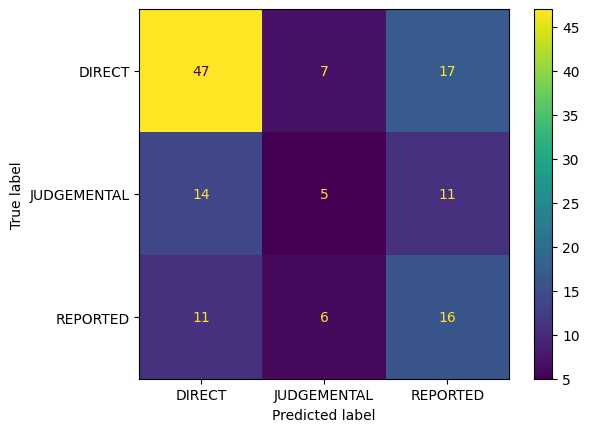
\includegraphics[width=10cm]{imagenes/Evaluacion/confusion_matrix/twitter_roberta_base_emotion-english-dirty_task2.png}
    \caption{\centering matriz de confusión para twitter\_roberta\_base\_emotion inglés}
\end{figure}

Lo primero que se puede observar de manera bastante clara es que el modelo tiene tendencia hacia la clase Direct de manera mayoritaria con un total de 47 instancias del total de 134 donde las siguientes clases son la Judgemental y Reported con un total de 18 y 44 respectivamente. De nuevo se observa esa tendencia a sobre clasificar una de las clases Judgemental o Reported por parte del modelo. En este caso Reported.

Por un lado, la primera clase tiene una tasa de acierto del 66.2\% donde las otras dos clases bajan radicalmente con unos valores del 16.7\% y 48.5\% respectivamente. Sin embargo, pese a estos valores tan bajos para ambas clases el modelo mantiene de manera global unos valores de tasa de acierto casualmente idénticos a los del modelo anterior con un 50.7\%.

Es decir, parece que efectivamente ese valor de loss tan dispar sugería correctamente que existía alguna tara con el modelo bert\_base\_uncased, concretamente parece que estaba sobreentrenado.

\subsection{Modelos bilingües}

A continuación, se realizará el análisis complementario, pero de los cuatro mejores modelos bilingües con el objetivo de determinar de nuevo sus capacidades, características y en general resultados respecto tanto de los modelos en inglés como de los modelos en la primera tarea.


\begin{table}[H]
\begin{tabular}{|l|l|l|l|l|}
\hline
\rowcolor[HTML]{9B9B9B} 
\multicolumn{1}{|c|}{\cellcolor[HTML]{9B9B9B}{\color[HTML]{000000} \textbf{Versión}}}           
& \multicolumn{1}{c|}{\cellcolor[HTML]{9B9B9B}{\color[HTML]{000000} \textbf{Accuracy}}} 
& \multicolumn{1}{c|}{\cellcolor[HTML]{9B9B9B}{\color[HTML]{000000} \textbf{F1}}} 
& \multicolumn{1}{c|}{\cellcolor[HTML]{9B9B9B}{\color[HTML]{000000} \textbf{Precision}}}
& \multicolumn{1}{c|}{\cellcolor[HTML]{9B9B9B}{\color[HTML]{000000} \textbf{Recall}}} 
\\ \hline
\rowcolor[HTML]{E7E6E6} 
\cellcolor[HTML]{9B9B9B}{\color[HTML]{000000} \textbf{bert\_base-cased}}                                                         
& {\color[HTML]{000000} 0.555}                                                     
& {\color[HTML]{000000} 0.463}                                            
& {\color[HTML]{000000} 0.495}                                                    
& {\color[HTML]{000000} 0.496}                                           
\\ \hline
\rowcolor[HTML]{E7E6E6} 
\cellcolor[HTML]{9B9B9B}{\color[HTML]{000000} \textbf{bert\_base\_multilingual-uncased}}                                             
& {\color[HTML]{000000} 0.587}                                                      
& {\color[HTML]{000000} 0.549}                                               
& {\color[HTML]{000000} 0.556}                                                        
& {\color[HTML]{000000} 0.561}                                                   
\\ \hline
\rowcolor[HTML]{E7E6E6} 
\cellcolor[HTML]{9B9B9B}{\color[HTML]{000000} \textbf{twitter\_roberta\_base\_emotion}}                                                   
& {\color[HTML]{000000} 0.590}                                                      
& {\color[HTML]{000000} 0.547}                                                
& {\color[HTML]{000000} 0.552}                                                  
& {\color[HTML]{000000} 0.548}                                                
\\ \hline
\rowcolor[HTML]{E7E6E6} 
\cellcolor[HTML]{9B9B9B}{\color[HTML]{000000} \textbf{XLM\_roBERTa}}                                                                   
& {\color[HTML]{000000} 0.580}                                                    
& {\color[HTML]{000000} 0.537}                                                
& {\color[HTML]{000000} 0.537}                                                  
& {\color[HTML]{000000} 0.548}                                                
\\ \hline
\end{tabular}
\caption{Métricas de los modelos bilingües segunda tarea.}
\end{table}

Lo primero que se puede observar es que los valores de accuracy son claramente inferiores a los de los modelos ingleses con un valor medio alrededor del 57.5\% frente al 60.5\% que mostraban los otros. En general resultados así son de esperar al tratarse de una tarea con mayor complejidad para los modelos de base debido a la mezcla de idiomas, siendo bert un sistema de modelos predominantemente en inglés. Sin embargo, habrá que estudiarlo más en profundidad.

Por un lado el modelo Twitter\_roberta\_base\_emotion aparece de nuevo con un valor de F1  de 0.547 situándose como segundo mejor modelo en esta categoría y con un accuracy del 0.59, en este caso como mejor modelo. En primer lugar, se encuentra el modelo bert\_base\_multilingual-uncased con un valor de F1 realmente similar de 0.549 y lo mismo para su accuracy con un valor de 0.587.

Para esta sección se van a comparar de nuevo dos modelos, concretamente los dos ya mencionados, en este caso por su extrema similitud en las métricas y adicionalmente debido a que el modelo Twitter\_roberta\_base\_emotion sigue siendo una buena comparativa al tratarse del mejor modelo en general hasta el momento durante todo el trabajo.

\subsection{Mejores modelos bilingües: Twitter\_roberta\_base\_emotion}

Estas secciones tienen como objetivo analizar las diferencias entre ambos modelos de tal manera que se puedan observar sus características internas más allá de sus resultados globales. En este caso no hubo ningún resultado anómalo durante el entrenamiento por lo que el estudio se centra en observar su comportamiento.

A continuación, se muestra la tabla con los diferentes resultados y métricas obtenidas:

\begin{table}[H]
\begin{tabular}{|l|c|c|c|c|}
\hline
\rowcolor[HTML]{9B9B9B} 
\multicolumn{1}{|c|}{\cellcolor[HTML]{9B9B9B}{\color[HTML]{000000} \textbf{Versión}}}
& \multicolumn{1}{l|}{\cellcolor[HTML]{9B9B9B}{\color[HTML]{000000} \textbf{Direct}}} 
& \multicolumn{1}{l|}{\cellcolor[HTML]{9B9B9B}{\color[HTML]{000000} \textbf{Judgemental}}} 
& \multicolumn{1}{l|}{\cellcolor[HTML]{9B9B9B}{\color[HTML]{000000} \textbf{Reported}}} 
& \multicolumn{1}{l|}{\cellcolor[HTML]{9B9B9B}{\color[HTML]{000000} \textbf{Average}}} 
\\ \hline
\rowcolor[HTML]{E7E6E6} 
\cellcolor[HTML]{9B9B9B}{\color[HTML]{000000} \textbf{F1}}                          
& {\color[HTML]{000000} 0.75}                                                        
& {\color[HTML]{000000} 0.37}                                                           
& {\color[HTML]{000000} 0.47}                                                           
& {\color[HTML]{000000} 0.60}                                            
\\ \hline
\rowcolor[HTML]{E7E6E6} 
\cellcolor[HTML]{9B9B9B}{\color[HTML]{000000} \textbf{Precision}}       
& {\color[HTML]{000000} 0.70}                                                        
& {\color[HTML]{000000} 0.33}                                                         
& {\color[HTML]{000000} 0.64}                                                           
& {\color[HTML]{000000} 0.62}                                                
\\ \hline
\rowcolor[HTML]{E7E6E6} 
\cellcolor[HTML]{9B9B9B}{\color[HTML]{000000} \textbf{Recall}}             
& {\color[HTML]{000000} 0.80}                                                     
& {\color[HTML]{000000} 0.43}                                                        
& {\color[HTML]{000000} 0.38}                                                           
& {\color[HTML]{000000} 0.61}                                          
\\ \hline
\end{tabular}
\caption{Métricas twitter\_roberta\_base\_emotion bilingüe.}
\end{table}

Inmediatamente se observan unos valores razonablemente buenos para la clase Direct de alrededor del 0.75 para las 3 métricas, lo cual representa los mejores resultados sobre el set de test hasta la fecha. Además, se ha observado que los resultados para las demás clases no son tan radicalmente malos como en los demás modelos con valores de F1, Precision y recall de 0.37, 0.33 y 0.43 respectivamente para Judgemental y de 0.47, 0.64 y 0.38 para Reported. 

A diferencia de en otros modelos, en esta tabla se observa algo más de equilibrio entre las dos clases minoritarias. Este factor puede deberse a que el modelo esta mejor entrenado bien sea por el mayor número de instancias o por el formato del dataset bilingüe.

En total estos resultados brindan alrededor de un 0.6 global de media ponderada para las 3 métricas en el set de test. Este resultado quedará contrastado una vez se realice un breve análisis de la matriz de confusión y se comparen las diferentes accuracy para las 3 clases.


\begin{figure}[H]
    \centering
    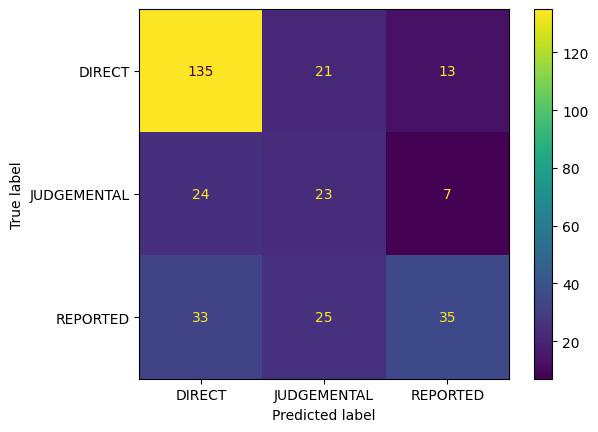
\includegraphics[width=10cm]{imagenes/Evaluacion/confusion_matrix/twitter_roberta_base_emotion-all-dirty.png}
    \caption{\centering matriz de confusión para twitter\_roberta\_base\_emotion bilingüe}
\end{figure}

Para la primera clase se observan buenos resultados con un total de 135 instancias bien clasificadas respecto de un total de 168 (un 80.36\%). Si bien la primera clase obtiene buenos resultados, las otras dos, Judgemental y Reported, no tanto. Por un lado, se tiene Judgemental con 23 instancias bien clasificadas (un 42.6\%) y por otro lado Reported con un total de 35 (un 37.63\%) instancias bien clasificadas.

En general este modelo parece mantener unos buenos resultados, mejores que ningún otro para como mínimo la primera de las clases y para las otras dos clases mantiene unos resultados bajos, pero en la media respecto de los otros modelos. Es decir, en general el modelo obtiene unos valores de accuracy del 61.08\%, siendo por tanto el mejor modelo hasta el momento analizado, aunque solo sea de manera general ya que realmente ese valor surge de los altos resultados para la clase Direct y no tanto para las otras dos clases como ya se ha comentado.


\subsection{Mejores modelos bilingües: Bert\_base\_multilingual-uncased}

Se estudia el siguiente modelo debido a sus resultados obtenidos en la fase previa y como comparativa respecto del modelo anterior. El objetivo es estudiar sus resultados y analizar su comportamiento para ver si se cumplen los mismos patrones que para modelos anteriores.

\begin{table}[H]
\begin{tabular}{|l|c|c|c|c|}
\hline
\rowcolor[HTML]{9B9B9B} 
\multicolumn{1}{|c|}{\cellcolor[HTML]{9B9B9B}{\color[HTML]{000000} \textbf{Versión}}} 
& \multicolumn{1}{l|}{\cellcolor[HTML]{9B9B9B}{\color[HTML]{000000} \textbf{Direct}}}
& \multicolumn{1}{l|}{\cellcolor[HTML]{9B9B9B}{\color[HTML]{000000} \textbf{Judgemental}}}
& \multicolumn{1}{l|}{\cellcolor[HTML]{9B9B9B}{\color[HTML]{000000} \textbf{Reported}}} 
& \multicolumn{1}{l|}{\cellcolor[HTML]{9B9B9B}{\color[HTML]{000000} \textbf{Average}}} 
\\ \hline
\rowcolor[HTML]{E7E6E6} 
\cellcolor[HTML]{9B9B9B}{\color[HTML]{000000} \textbf{F1}}                         
& {\color[HTML]{000000} 0.71 }                                            
& {\color[HTML]{000000} 0.27 }                                                        
& {\color[HTML]{000000} 0.63 }                                                          
& {\color[HTML]{000000} 0.61 }                                             
\\ \hline
\rowcolor[HTML]{E7E6E6} 
\cellcolor[HTML]{9B9B9B}{\color[HTML]{000000} \textbf{Precision}}                  
& {\color[HTML]{000000} 0.74 }                                                        
& {\color[HTML]{000000} 0.26 }                                                       
& {\color[HTML]{000000} 0.60 }                                                         
& {\color[HTML]{000000} 0.62 }                                                
\\ \hline
\rowcolor[HTML]{E7E6E6} 
\cellcolor[HTML]{9B9B9B}{\color[HTML]{000000} \textbf{Recall}}              
& {\color[HTML]{000000} 0.69 }                                                      
& {\color[HTML]{000000} 0.28 }                                                        
& {\color[HTML]{000000} 0.67 }                                                            
& {\color[HTML]{000000} 0.61 }                                                       
\\ \hline
\end{tabular}
\caption{Métricas segunda tarea bert\_base\_multilingual-uncased.}
\end{table}

En primer lugar, se observa de manera clara de nuevo que la clase Direct es la clase con mejores resultados de las 3, sin embargo de manera atípica, la clase Reported no se encuentran lejos con un valor de F1 de 0.63 respecto del 0.71 de la clase Direct.

Por otro lado, la clase Judgemental obtiene unos valores bajísimos para las 3 métricas con 0.27, 0.26 y 0.28 respectivamente para F1, Precision y recall. Esto va en concordancia con la hipótesis de que al ser dos clases muy similares los modelos iban a tener problemas a la hora de diferenciarlas y tenderían a una de las dos como ya se ha observado en anteriores modelos durante el análisis de la tarea 2.

Para poder tener una perspectiva más clara se va a observar la matriz de confusión generada por el modelo:

\begin{figure}[H]
    \centering
    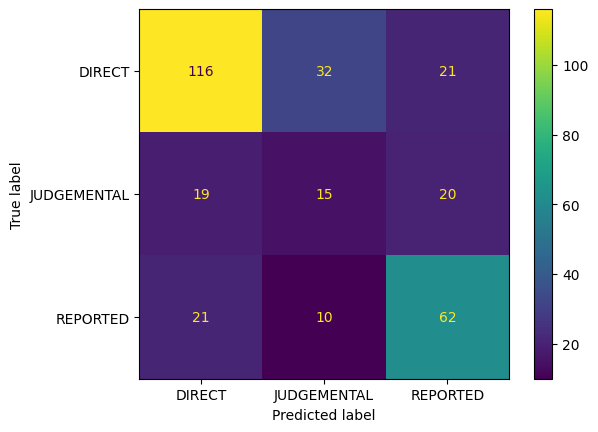
\includegraphics[width=10cm]{imagenes/Evaluacion/confusion_matrix/bert_base_multilingual-uncased-all-dirty_task2.png}
    \caption{\centering matriz de confusión para bert\_base\_multilingual-uncased}
\end{figure}

Como ya se comentaba tanto la clase Direct como la clase Reported obtienen buenos resultados con 116 y 62 instancias correctamente clasificadas para ambas clases frente a las solo 15 de la clase Judgemental.

Es decir, a diferencia del anterior modelo este obtiene valores más bajos para la clase Direct con 116 instancias de 169 (un 68,6\%) pero lo compensa con unos resultados mucho mejores para la clase Reported con 62 instancias de 93 (un 66,6\%) aunque es cierto que para la clase Judgemental cae con un total de 15 instancias de (un 27,7\%).

De nuevo se observa el patrón de clasificación para las dos clases Judgemental y Reported, generando un modelo que tiende a clasificar como una de las dos clases la mayor parte de las instancias de ambas.


\section{Conclusiones modelos}

Finalmente se va a dedicar una sección a cerrar los análisis de ambas tareas determinando que modelos son los mejores y que problemas y limitaciones se han ido encontrando. Si bien se pretende realizar unas conclusiones, estas solo serán sobre los modelos ya que las conclusiones del trabajo se realizarán al final de este.


\subsection{Primera tarea}

En primera instancia se decidió subdividir la tarea en dos versiones, una con un dataset solo con tweets en inglés y otra con todos los tweets (español e inglés), de tal manera que se pudiera observar cuales eran las diferencias entre ambas aproximaciones y ver que alcance tenían los diferentes modelos bert al enfrentarse a una tarea bilingüe.

Además del enfoque por idiomas también se planteó una subdivisión en base al preprocesamiento con el objetivo de observar si aplicar preprocesamiento a los textos mejoraba o empeoraba los resultados finales de los modelos. 

En general y de manera resumida se observó claramente que los modelos con preprocesamiento obtenían peores resultados que aquellos que no estaban preprocesados. Esto se puede deber a diversos factores desde la posibilidad de haber realizado un preprocesamiento que no favorezca si no que perjudique a los modelos hasta la conclusión de que preprocesar los textos hace que el tokenizador no recoja información que de otra manera si recoge y se pierda parte de esa información y por ende de su capacidad de clasificación. Esto se planteará en mejoras futuras.

Como se esperaba la tarea en inglés obtuvo mejores resultados en general convergiendo en el modelo generado con la variante twitter-roberta-base-emotion de roberta para la que se obtuvo un 81.06\% para la tarea 1. Este resultado se sitúa de hecho como el mejor resultado obtenido en todo el trabajo y sería el modelo final si no fuera por su limitación a la hora de trabajar con tweets en español.

Por ello se generó y estudió como ya se comentó una serie de modelos usando el dataset entero con el objetivo de poder realizar la tarea al completo. Para esta tarea se esperaban resultados significativamente peores que los obtenidos para la tarea únicamente inglesa.

Sin embargo, los resultados no son tan malos como se esperaba, convergiendo finalmente en el modelo generado con bert-multilingual-uncased con una tasa de acierto del 77.76\%.

Cabe destacar que si bien ambos modelos generan buenos resultados tienen ambos una tendencia a sobre clasificar hacia la clase No Sexista respecto de la Sexista. Esto probablemente se deba a su el desbalance de los datos del dataset y se deberá plantear en mejoras a futuro.


\subsection{Segunda tarea}

La segunda tarea tenía como objetivo realizar un estudio simplificado de las capacidades de los modelos bert, utilizando como ejemplo los mejores modelos de la anterior tarea. Si bien se sabe que esta aproximación no garantiza los mejores resultados sirve para hacer un estudio de la capacidad de generalizar de esos modelos.

En primera instancia se realizó un estudio con los modelos basados en el dataset en inglés para los que se obtuvieron resultados en general negativos y especialmente para las clases Judgemental y Reported, resultados bastante bajos. específicamente estas dos clases se plantearon de base como una muy probable problemática debido a sus grandes similitudes y discrepancias por parte de los propios anotadores durante todo el dataset. De hecho, se ejemplificó como para un mismo tweet era común encontrar división entre estas dos clases.

Una vez estudiados los diferentes modelos se alcanzó una conclusión sobre ellos, obteniendo para el modelo generado con twitter-roberta-base-emotion una tasa de acierto del 50\%. 

Para la segunda tanda de modelos se esperaba un comportamiento similar a la primera tarea, empeorando de forma ligera los resultados respecto de sus contrapartes en inglés. Sin embargo, los modelos bilingües obtuvieron para las pruebas sobre el test set unos resultados sorprendentemente mejores. Concretamente la tasa de acierto para twitter-roberta-base-emotion y XML-roberta fueron para ambos de un 60\%.

Probablemente estos resultados se deban al reducido tamaño del set de test por lo que con poco los resultados cambian radicalmente y no tanto a un factor de mejor entrenamiento, pero aun así es muy interesante observar cómo su comportamiento difirió completamente de lo esperado para ellos. De nuevo se deberá incluir en mejoras a futuro aumentar el set de test para obtener pruebas con valores más representativos.